\documentclass{anstrans}

\title{SAFETY ANALYSIS OF THE MOLTEN SALT FAST REACTOR FUEL COMPOSITION USING
MOLTRES \\ \textit{(Preprint submitted to ANS Global 2019 International Fuel
Cycle Conference)} \\~\\~\\}
\author{Sun Myung Park$^{a,b}$, Andrei Rykhlevskii$^a$, and
Kathryn D. Huff$^a$}
\institute{$^a$Dept. of Nuclear, Plasma and Radiological Engineering,
University of Illinois at Urbana-Champaign}
\email{$^b$smpark3@illinois.edu}

\usepackage{graphicx} % allows inclusion of graphics
%\usepackage{booktabs} % nice rules (thick lines) for tables
\usepackage{microtype} % improves typography for PDF
\usepackage{float}
\usepackage{longtable}
\usepackage{xspace}
\usepackage{multirow} 
\usepackage{array}
\setlength{\arrayrulewidth}{.4mm}
\renewcommand{\arraystretch}{1.2}
\usepackage[labelfont=bf]{caption}
\usepackage{caption}
\usepackage{subcaption}
\usepackage{enumitem}
\usepackage{placeins}
\usepackage{siunitx}
%\newcolumntype{c}{>{\hsize=.56\hsize}X}
%\newcolumntype{b}{>{\hsize=.7\hsize}X}
%\newcolumntype{s}{>{\hsize=.74\hsize}X}
%\newcolumntype{f}{>{\hsize=.1\hsize}X}
%\newcolumntype{a}{>{\hsize=.45\hsize}X}
%\usepackage{titlesec}
%\titleformat*{\subsection}{\normalfont}
%\usepackage[super]{cite}
\usepackage{multirow}
\usepackage{hhline}
\usepackage{dcolumn}


\usepackage[acronym,toc]{glossaries}
%\newacronym{<++>}{<++>}{<++>}
\newacronym[longplural={metric tons of heavy metal}]{MTHM}{MTHM}{metric ton of heavy metal}
\newacronym{ABM}{ABM}{agent-based modeling}
\newacronym{ACDIS}{ACDIS}{Program in Arms Control \& Domestic and International Security}
\newacronym{AHTR}{AHTR}{Advanced High Temperature Reactor}
\newacronym{ANDRA}{ANDRA}{Agence Nationale pour la gestion des D\'echets RAdioactifs, the French National Agency for Radioactive Waste Management}
\newacronym{ANL}{ANL}{Argonne National Laboratory}
\newacronym{API}{API}{application programming interface}
\newacronym{ARE}{ARE}{Aircraft Reactor Experiment}
\newacronym{ARFC}{ARFC}{Advanced Reactors and Fuel Cycles}
\newacronym{ASME}{ASME}{American Society of Mechanical Engineers}
\newacronym{ATWS}{ATWS}{Anticipated Transient Without Scram}
\newacronym{BDBE}{BDBE}{Beyond Design Basis Event}
\newacronym{BIDS}{BIDS}{Berkeley Institute for Data Science}
\newacronym{BOL}{BOL}{beginning of life}
\newacronym{CAFCA}{CAFCA}{ Code for Advanced Fuel Cycles Assessment }
\newacronym{CDTN}{CDTN}{Centro de Desenvolvimento da Tecnologia Nuclear}
\newacronym{CEA}{CEA}{Commissariat \`a l'\'Energie Atomique et aux \'Energies Alternatives}
\newacronym{CI}{CI}{continuous integration}
\newacronym{CNEN}{CNEN}{Comiss\~{a}o Nacional de Energia Nuclear}
\newacronym{CNERG}{CNERG}{Computational Nuclear Engineering Research Group}
\newacronym{COSI}{COSI}{Commelini-Sicard}
\newacronym{COTS}{COTS}{commercial, off-the-shelf}
\newacronym{CSNF}{CSNF}{commercial spent nuclear fuel}
\newacronym{CTAH}{CTAHs}{Coiled Tube Air Heaters}
\newacronym{CUBIT}{CUBIT}{CUBIT Geometry and Mesh Generation Toolkit}
\newacronym{CURIE}{CURIE}{Centralized Used Fuel Resource for Information Exchange}
\newacronym{DAG}{DAG}{directed acyclic graph}
\newacronym{DANESS}{DANESS}{Dynamic Analysis of Nuclear Energy System Strategies}
\newacronym{DBE}{DBE}{Design Basis Event}
\newacronym{DESAE}{DESAE}{Dynamic Analysis of Nuclear Energy Systems Strategies}
\newacronym{DHS}{DHS}{Department of Homeland Security}
\newacronym{DOE}{DOE}{Department of Energy}
\newacronym{DRACS}{DRACS}{Direct Reactor Auxiliary Cooling System}
\newacronym{DRE}{DRE}{dynamic resource exchange}
\newacronym{DSNF}{DSNF}{DOE spent nuclear fuel}
\newacronym{DYMOND}{DYMOND}{Dynamic Model of Nuclear Development }
\newacronym{EBS}{EBS}{Engineered Barrier System}
\newacronym{EDZ}{EDZ}{Excavation Disturbed Zone}
\newacronym{EIA}{EIA}{U.S. Energy Information Administration}
\newacronym{EOL}{EOL}{end of life}
\newacronym{EPA}{EPA}{Environmental Protection Agency}
\newacronym{EP}{EP}{Engineering Physics}
\newacronym{FCO}{FCO}{Fuel Cycle Options}
\newacronym{FCT}{FCT}{Fuel Cycle Technology}
\newacronym{FEHM}{FEHM}{Finite Element Heat and Mass Transfer}
\newacronym{FEPs}{FEPs}{Features, Events, and Processes}
\newacronym{FHR}{FHR}{Fluoride-Salt-Cooled High-Temperature Reactor}
\newacronym{FLiBe}{FLiBe}{Fluoride-Lithium-Beryllium}
\newacronym{GDSE}{GDSE}{Generic Disposal System Environment}
\newacronym{GDSM}{GDSM}{Generic Disposal System Model}
\newacronym{GENIUSv1}{GENIUSv1}{Global Evaluation of Nuclear Infrastructure Utilization Scenarios, Version 1}
\newacronym{GENIUSv2}{GENIUSv2}{Global Evaluation of Nuclear Infrastructure Utilization Scenarios, Version 2}
\newacronym{GENIUS}{GENIUS}{Global Evaluation of Nuclear Infrastructure Utilization Scenarios}
\newacronym{GPAM}{GPAM}{Generic Performance Assessment Model}
\newacronym{GRSAC}{GRSAC}{Graphite Reactor Severe Accident Code}
\newacronym{GUI}{GUI}{graphical user interface}
\newacronym{HLW}{HLW}{high level waste}
\newacronym{HPC}{HPC}{high-performance computing}
\newacronym{HTC}{HTC}{high-throughput computing}
\newacronym{HTGR}{HTGR}{High Temperature Gas-Cooled Reactor}
\newacronym{IAEA}{IAEA}{International Atomic Energy Agency}
\newacronym{IEMA}{IEMA}{Illinois Emergency Mangament Agency}
\newacronym{INL}{INL}{Idaho National Laboratory}
\newacronym{IPRR1}{IRP-R1}{Instituto de Pesquisas Radioativas Reator 1}
\newacronym{IRP}{IRP}{Integrated Research Project}
\newacronym{ISFSI}{ISFSI}{Independent Spent Fuel Storage Installation}
\newacronym{ISRG}{ISRG}{Independent Student Research Group}
\newacronym{JFNK}{JFNK}{Jacobian-Free Newton Krylov}
\newacronym{LANL}{LANL}{Los Alamos National Laboratory}
\newacronym{LBNL}{LBNL}{Lawrence Berkeley National Laboratory}
\newacronym{LCOE}{LCOE}{levelized cost of electricity}
\newacronym{LDRD}{LDRD}{laboratory directed research and development}
\newacronym{LFR}{LFR}{Lead-Cooled Fast Reactor}
\newacronym{LLNL}{LLNL}{Lawrence Livermore National Laboratory}
\newacronym{LMFBR}{LMFBR}{Liquid Metal Fast Breeder Reactor}
\newacronym{LOFC}{LOFC}{Loss of Forced Cooling}
\newacronym{LOHS}{LOHS}{Loss of Heat Sink}
\newacronym{LOLA}{LOLA}{Loss of Large Area}
\newacronym{LP}{LP}{linear program}
\newacronym{LWR}{LWR}{Light Water Reactor}
\newacronym{MA}{MA}{minor actinide}
\newacronym{MCNP}{MCNP}{Monte Carlo N-Particle code}
\newacronym{MILP}{MILP}{mixed-integer linear program}
\newacronym{MIT}{MIT}{the Massachusetts Institute of Technology}
\newacronym{MOAB}{MOAB}{Mesh-Oriented datABase}
\newacronym{MOOSE}{MOOSE}{Multiphysics Object-Oriented Simulation Environment}
\newacronym{MOX}{MOX}{mixed oxide}
\newacronym{MSBR}{MSBR}{Molten Salt Breeder Reactor}
\newacronym{MSFR}{MSFR}{Molten Salt Fast Reactor}
\newacronym{MSRE}{MSRE}{Molten Salt Reactor Experiment}
\newacronym{MSR}{MSR}{Molten Salt Reactor}
\newacronym{NAGRA}{NAGRA}{National Cooperative for the Disposal of Radioactive Waste}
\newacronym{NEAMS}{NEAMS}{Nuclear Engineering Advanced Modeling and Simulation}
\newacronym{NEUP}{NEUP}{Nuclear Energy University Programs}
\newacronym{NFCSim}{NFCSim}{Nuclear Fuel Cycle Simulator}
\newacronym{NGNP}{NGNP}{Next Generation Nuclear Plant}
\newacronym{NMWPC}{NMWPC}{Nuclear MW Per Capita}
\newacronym{NNSA}{NNSA}{National Nuclear Security Administration}
\newacronym{NPRE}{NPRE}{Department of Nuclear, Plasma, and Radiological Engineering}
\newacronym{NQA1}{NQA-1}{Nuclear Quality Assurance - 1}
\newacronym{NRC}{NRC}{Nuclear Regulatory Commission}
\newacronym{NSF}{NSF}{National Science Foundation}
\newacronym{NSSC}{NSSC}{Nuclear Science and Security Consortium}
\newacronym{NUWASTE}{NUWASTE}{Nuclear Waste Assessment System for Technical Evaluation}
\newacronym{NWF}{NWF}{Nuclear Waste Fund}
\newacronym{NWTRB}{NWTRB}{Nuclear Waste Technical Review Board}
\newacronym{OCRWM}{OCRWM}{Office of Civilian Radioactive Waste Management}
\newacronym{ORION}{ORION}{ORION}
\newacronym{ORNL}{ORNL}{Oak Ridge National Laboratory}
\newacronym{PARCS}{PARCS}{Purdue Advanced Reactor Core Simulator}
\newacronym{PBAHTR}{PB-AHTR}{Pebble Bed Advanced High Temperature Reactor}
\newacronym{PBFHR}{PB-FHR}{Pebble-Bed Fluoride-Salt-Cooled High-Temperature Reactor}
\newacronym{PEI}{PEI}{Peak Environmental Impact}
\newacronym{PH}{PRONGHORN}{PRONGHORN}
\newacronym{PRKE}{PRKE}{Point Reactor Kinetics Equations}
\newacronym{PSPG}{PSPG}{Pressure-Stabilizing/Petrov-Galerkin}
\newacronym{PWAR}{PWAR}{Pratt and Whitney Aircraft Reactor}
\newacronym{PWR}{PWR}{Pressurized Water Reactor}
\newacronym{PyNE}{PyNE}{Python toolkit for Nuclear Engineering}
\newacronym{PyRK}{PyRK}{Python for Reactor Kinetics}
\newacronym{QA}{QA}{quality assurance}
\newacronym{RDD}{RD\&D}{Research Development and Demonstration}
\newacronym{RD}{R\&D}{Research and Development}
\newacronym{RELAP}{RELAP}{Reactor Excursion and Leak Analysis Program}
\newacronym{RIA}{RIA}{Reactivity Insertion Accident}
\newacronym{RIF}{RIF}{Region-Institution-Facility}
\newacronym{SFR}{SFR}{Sodium-Cooled Fast Reactor}
\newacronym{SINDAG}{SINDA{\textbackslash}G}{Systems Improved Numerical Differencing Analyzer $\backslash$ Gaski}
\newacronym{SKB}{SKB}{Svensk K\"{a}rnbr\"{a}nslehantering AB}
\newacronym{SNF}{SNF}{spent nuclear fuel}
\newacronym{SNL}{SNL}{Sandia National Laboratory}
\newacronym{STC}{STC}{specific temperature change}
\newacronym{SUPG}{SUPG}{Streamline-Upwind/Petrov-Galerkin}
\newacronym{SWF}{SWF}{Separations and Waste Forms}
\newacronym{SWU}{SWU}{Separative Work Unit}
\newacronym{TRIGA}{TRIGA}{Training Research Isotope General Atomic}
\newacronym{TRISO}{TRISO}{Tristructural Isotropic}
\newacronym{TSM}{TSM}{Total System Model}
\newacronym{TSPA}{TSPA}{Total System Performance Assessment for the Yucca Mountain License Application}
\newacronym{ThOX}{ThOX}{thorium oxide}
\newacronym{UFD}{UFD}{Used Fuel Disposition}
\newacronym{ULOHS}{ULOHS}{Unprotected Loss of Heat Sink}
\newacronym{UML}{UML}{Unified Modeling Language}
\newacronym{UOX}{UOX}{uranium oxide}
\newacronym{UQ}{UQ}{uncertainty quantification}
\newacronym{US}{US}{United States}
\newacronym{UW}{UW}{University of Wisconsin}
\newacronym{VISION}{VISION}{the Verifiable Fuel Cycle Simulation Model}
\newacronym{VV}{V\&V}{verification and validation}
\newacronym{WIPP}{WIPP}{Waste Isolation Pilot Plant}
\newacronym{YMR}{YMR}{Yucca Mountain Repository Site}

\makeglossaries

\begin{document}

\begin{abstract}
%
\textit{
    The Molten
    Salt Fast Reactor (MSFR) has garnered much interest for its inherent
    safety and sustainbility features. The MSFR can adopt a closed thorium fuel
    cycle for
    sustainable operation through the breeding of $^{233}$U from $^{232}$Th.
    The fuel composition changes significantly over the course of its lifespan.
    In this study, we investigated the steady state and transient behavior of
    the MSFR using Moltres, a coupled neutronics/thermal-hydraulics code
    developed within the Multiphysics Object Oriented Simulation Environment
    (MOOSE) framework. Three different fuel compositions, start-up,
    early-life, and equilibrium, were examined for potentially
    dangerous
    core temperature excursions during a unprotected loss of heat sink (ULOHS)
    accident. The six-group and total neutron flux distributions 
    showed good agreement with SERPENT and
    published MSFR results, while the temperature distribution and total power
    showed discrepancies which can be attributed to known sources of error.
    For the transient behavior under the ULOHS
    scenario, while the transition time towards the new steady state core
    temperature is also in good agreement with existing MSFR simulations by
    Fiorina et al., Moltres underestimated the
    temperature rise by a factor of ten, due to the same sources of
    error affecting the steady state results. While an MSFR loaded with
    start-up fuel composition operates at a higher temperature than with the
    other two fuel compositions, all three cases were shown to be inherently
    safe due to the strong negative temperature feedback.
}
\end{abstract}

\section{Introduction}

	\glspl{MSR} are a class of nuclear reactors that
	contain nuclear fuel dissolved and circulating in a molten salt coolant
	loop.
	They potentially possess the ability to run for extended 
    periods with minimal shutdown time due to online fuel reprocessing.
    Their equilibrium fuel compositions differ substantially from
    start-up compositions not only due to burnup of initial fissile material
    and breeding of new fissile material, but also fissile material feeds and 
    removal of fission products. Also, while early-life fuel composition is
    largely dependent on the initial core loading, the long-term equilibrium
    fuel composition is determined by the type of feed.
    Since the changing fuel composition 
    impacts safety parameters (e.g. reactivity feedback coefficients), a 
    licensing case for this class of reactors  must fully characterize 
    those impacts.

	While numerous computational tools exist for conventional nuclear reactors, 
    \glspl{MSR} present unique computational challenges that many fail to 
    address effectively. \glspl{MSR} differ
    profoundly from conventional 
    solid-fuelled reactors, particularly in their neutronics and 
    thermal-hydraulics behaviors.  New \gls{MSR} simulation tools must 
    capture strong coupling between neutronics and thermal-hydraulics 
    exhibited by \gls{DNP} movement as well as strong 
    Doppler and density feedback in the fuel salt.  This paper investigates 
    the impact of changing fuel composition on fuel salt temperatures in the 
    \gls{MSFR} concept using a new simulation tool for \glspl{MSR}, Moltres 
    \cite{lindsay_introduction_2018}.
    
    Moltres is an open source coupled neutronics/thermal hydraulics simulation 
    application for simulating \glspl{MSR}. Built on the \gls{MOOSE} finite 
    element framework \cite{gaston_moose:_2009}, Moltres solves the coupled 
    time-dependent multi-group neutron diffusion, temperature, and 
    \gls{DNP} governing equations.  The temperature and \gls{DNP} equations
    fully account for flow via fuel salt advection.
    
    The \gls{MSFR} model studied in this paper is a reference design for a 
    fast-spectrum \gls{MSR} developed under H2020
    \gls{SAMOFAR} project \cite{gerardin_design_nodate}.
    The \gls{MSFR} boasts several safety and sustainability advantages over
    conventional reactors. Firstly, it can run on a closed thorium fuel cycle,
    which reduces actinide production and waste radiotoxity.
    The fast neutron spectrum improves $^{233}$U breeding from $^{232}$Th, an
    isotope that is approximately three times as abundant as uranium.
    Lastly, the \gls{MSFR} operates at near atmospheric pressure; this reduces
    the risk of containment structure failure and manufacturing costs.
    
    This paper presents results from Moltres simulations of the 
    \gls{MSFR} reference model with three fuel compositions:
    start-up, early-life, and equilibrium. In line with the purpose of the
    \gls{MSFR} as a thorium breeder, the chosen start-up fuel composition
    under study is a eutectic mixture of $^{233}$U and 
    $^{232}$Th fluorides in a lithium fluoride molten salt, with
    a Th/$^{233}$U mixture feed. $^{233}$U is extracted from
    the blanket tank and reinserted into the core
    \cite{merle-lucotte_launching_2011}.
    
    We generated group constants for 
    each fuel composition using SERPENT \cite{leppanen_serpent_2015}, a 
    continuous-energy Monte Carlo code for numerous reactor physics 
    applications. The group constants relevant for Moltres simulations are
    the various macroscopic neutron cross sections, neutron diffusion
    coefficient, average fission energy, average neutron yield, inverse
    neutron speed, fission spectrum, \gls{DNP} decay constants, and effective
    delayed neutron fractions.
    Using these group constants, Moltres then 
    solves for the flux and temperature based on the neutron diffusion 
    equation coupled with temperature advection due to coolant flow. Transient 
    simulations will establish core fuel temperatures during transients.
    These distributions will give insight into \gls{MSFR} transient behavior,
    which will help us identify potential safety risks.
    
\begin{figure}[h] 
	\centering
	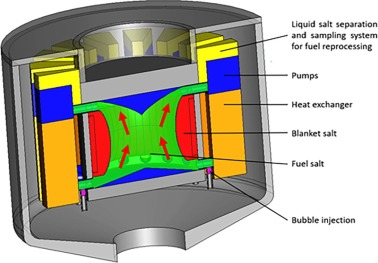
\includegraphics[width=0.48\textwidth]{./figures/MSFR}
	\caption{MSFR reactor design concept \cite{serp_molten_2014}.}
	\label{fig:msfr}
\end{figure} 

\begin{table}[h]
	\caption{Specifications of the \gls{MSFR} design \cite{serp_molten_2014}.}
	\begin{tabular}{ l l }
		\hline
		Parameter & Value \\
		\hline
		Thermal/Electric output [MW$_{\text{th}}$/MW$_{\text{e}}$] & 3000 /
		1500 
		\\
		Salt volume [m$^3$] & 18 \\
		Salt fraction in core & 0.5 \\
		Number of circulation loops & 16 \\
		Nominal flow rate [kg s$^{-1}$] & 18500  \\
		Nominal circulation time [s] & 4.0 \\
		Inlet/outlet temperature [K] & 923 / 1023 \\
		Blanket volume [m$^3$] & 7.3\\
		\hline
	\end{tabular}
	\label{table:msfr}
\end{table}

\begin{table}[t]
\centering
\captionsetup{justification=centering}
\caption{Fuel salt composition used for the Serpent simulation.}
\begin{tabular}{lS}
\hline
{Isotope} & {Mole fraction [\%]}\\
\hline
$^7$Li & 29.0\\
$^{19}$F & 62.6\\
$^{232}$Th & 7.40\\
$^{233}$U & 1.00\\
\hline
\end{tabular}
\label{table:fuelsalt}
\vspace{.5cm}
	\centering
	\captionsetup{justification=centering}
	\caption{Fuel and blanket salt properties. $T$ denotes temperature in
	Kelvins.}
	{\small
	\begin{tabular}{ll}
		\hline
		{Property} & {Value}\\
		\hline
		Density, $\rho$ [kg m$^{-3}$] & $4983.56 - 0.882 \cdot T$ \\
		Thermal cond. , $k$ [W m$^{-1}$ K$^{-1}$] & $0.928 + 8.397 \times 10
		^{-5} \cdot T$\\
		Specific heat, $c_p$ [J kg$^{-1}$ K$^{-1}$] & $-1111 + 2.78 \cdot T$ \\
		\hline
	\end{tabular}
	}
	\vspace{.5cm}
	\label{table:saltprop}
	\centering
	\captionsetup{justification=centering}
	\caption{Material compositions and densities of the absorber,
	and reflector regions. All elements listed are in their natural
	compositions.}
	{\small
	\begin{tabular}{llSr}
		\hline
		Region & Element & At\% & Density [kg m$^{-3}$]\\
		\hline
		\multirow{2}{*}{Absorber} & B & 80  & \multirow{2}{*}{2520}\\
		& C & 20 & \\
		\hline
		\multirow{4}{*}{Reflector} & Ni & 67.7 & \multirow{4}{*}{10000} \\
		& W & 25.0 & \\
		& Cr & 7.0 & \\
		& Al & 0.3 & \\
		\hline
	\end{tabular}
	}
	\label{table:material}
\end{table}
    
    Section II provides the specifications and a literature review of the
    \gls{MSFR} concept. Section III covers the overall modeling approach with
    respect to the codes used in this study: SERPENT and Moltres. Section IV
    presents steady state neutron flux and temperature distribution results
    from Moltres for the three different fuel compositions studied. Section V
    explores the \gls{MSFR}'s neutronic and thermodynamic response to a
    \gls{ULOHS} scenario. Lastly, Section VI provides conclusions and
    suggestions for future work.

\section{Molten Salt Fast Reactor}

	Figure \ref{fig:msfr} shows a schematic view of the \gls{MSFR}. The main
	specifications of the \gls{MSFR} are given in Table \ref{table:msfr}.

	Lithium fluoride (LiF) is the major component of the fuel and blanket
	molten salts used for the \gls{MSFR}. Fissile and fertile isotopes are
	introduced
	into the mixture by mole fractions of 77.5\%LiF-22.5\%AcF$_4$, where
	AcF$_4$ represents actinide fluorides such as uranium and thorium
	fluorides. Table \ref{table:fuelsalt} shows the mole fraction of the
	molecular constituents in the \gls{MSFR} fuel salt, with the relevant
	physical properties in Table \ref{table:saltprop}.
	The \gls{MSFR} supports various fuel compositions; it can run on the same 
	$^{235}$U-$^{238}$U fuel used in most conventional LWRs. It can also run
	on a
	mixture of fresh and used uranium fuel containing reprocessed TRU
	isotopes \cite{fiorina_investigation_2013}. However, the main configuration
	of the \gls{MSFR} is a breeder reactor running on $^{233}$U-$^{232}$Th
	\cite{merle-lucotte_launching_2011}. Previous studies have reported
	breeding ratios of up to 1.1 on the \gls{MSFR} \cite{fiorina_molten_2013}. 

	The primary fuel salt flows upwards through the 9 m$^3$ central core
	region. At the top of the core, the flow separates into 16 smaller external
	loops, each of which passes through a heat exchanger and is pumped back
	into the core. The primary heat exchangers transfer heat from the fuel salt 
	to an intermediate salt coolant loop. There is other instrumentation along
	the external loops for online reprocessing and gas sparging. The core is
	radially surrounded by a tank of blanket molten salt, with reflectors at
	the top and bottom of the core. The blanket salt contains fertile isotopes
	such as $^{232}$Th for fuel breeding. There is a layer of neutron absorbing
	material behind the blanket tanks to protect the heat exchangers, pumps and
	other instrumentation from neutron irradiation damage.

	Various authors have performed a number of steady state and transient
	multiphysics simulations for the \gls{MSFR}. A paper by Fiorina et al.
	\cite{fiorina_modelling_2014} compares results between models
	developed on the multiphysics software COMSOL, and coupled in-house codes
	developed at
	Delft University of Technology. The models used 2D axisymmetric models of
	the \gls{MSFR} and solved multi-group neutron diffusion equations for the
	neutronics, and they showed good agreement for some of the transient cases
	studied. A more comprehensive 3D model has been developed and studied by
	Aufiero et al. \cite{aufiero_development_2014} using the computional fluid
	dynamics (CFD) toolbox OpenFOAM. Although this model relied on the one
	group neutron diffusion equation, it enabled the study of the full 3D core
	geometry and 3D transient scenarios such as the failure of one of the 16
	pumps in the \gls{MSFR}.

	More recently, a coupled tool, comprising of the thermal-hydraulics code
	TRACE and a multi-group 3D spatial neutronics solver \gls{PARCS}, was
	used to run steady state and transient simulations of the \gls{MSFR}
	\cite{pettersen_coupled_2016}. As \gls{PARCS} only supports conventional
	fuel assembly shapes, the authors approximated the 3D axisymmetric
	cylindrical \gls{MSFR} model with
	hexagonal fuel assemblies. This approach allowed for a 3D model
	simulation of the \gls{MSFR} on a coarse mesh and showed good agreement
	with the COMSOL and TUDelft models with the benefit of much lower
	computation times in comparison to the OpenFOAM CFD model. On top of
	steady state simulations, the transient scenarios studied by Pettersen
	include loss of heat sink, pump over-speed, over-cooling and loss of flow.
	
	As Moltres is developed on the \gls{MOOSE} framework, it can perform
	implicit multiphysics coupling on an adaptive meshing scheme over multiple
	processing units for accurate and efficient \gls{MSR} simulations.
	This paper aims to present Moltres simulation results and safety analysis
	of the \gls{MSFR}, for various fuel compositions through its operational
	lifetime. 

\section{Methodology}

	This section describes the overall modelling approach and the codes used
	in this paper. First, the early-life and equilibrium compositions were
	obtained from SCALE/TRITON unit cell depletion calculations by Rykhlevskii
	et al. \cite{rykhlevskii_fuel_2019} The authors used unit cell
	approximations for the modeling
	fuel cycle performance of the \gls{MSFR} and three other fast-spectrum
	\glspl{MSR}. We selected the equilibrium composition at
	approximately 43 years after start-up because the TRU vector change
	between each depletion time-step from this moment onwards is less than 3\%
	\cite{rykhlevskii_fuel_2019}. For the early-life composition, it is the 
	resulting fuel composition at 300 days after start-up.
	
	We performed neutronics calculations on SERPENT using these fuel
	compositions and a truncated, reference \gls{MSFR} core model
	\cite{pettersen_coupled_2016} to generate six-group neutronics data for
	Moltres. The material compositions and densities for the absorber,
	and reflector regions are given in Table \ref{table:material}. We set a
	neutron population of 200,000 with 50 inactive cycles and 500 active
	cycles. For
	simplicity, the heat exchanger and pump region were modeled after
	Hastelloy N \cite{hastelloy_2017}. Isotopes in the fuel compositions, whose
	neutron cross-section data are not found in the
	JEFF-3.1.2 nuclear data library, were omitted from these calculations
	The energy boundaries for the six neutron groups were adopted from previous
	\gls{MSFR} studies and shown in Table \ref{table:bound}.
	As for the \gls{DNP}, there are eight \gls{DNP} groups implicitly defined
	by the JEFF-3.1.2 nuclear data library.
	The reactor model is a 2D axisymmetric model as shown in
	Figure \ref{fig:reference}. This geometry focuses on the active central
	region of the core. Basing the geometry on the reference model facilitates
	comparisons with previous MSFR studies by various authors
	\cite{fiorina_modelling_2014} \cite{pettersen_coupled_2016} on the
	reference model for code-to-code verification purposes.
	The 2D model is extended into a 3D model in SERPENT by rotating it
	around the central axis to form concentric cylinders. Table
	\ref{table:reactivity} shows the overall temperature reactivity feedback
	coefficients due to the Doppler effect and
	temperature-driven fuel salt expansion. The coefficients were derived by
	applying a least squares best fit on the multiplication factors at
	temperatures from 900 K to 1200 K with 50 K intervals.
	
\begin{table}[t]
	\centering
	\captionsetup{justification=centering}
	\caption{Neutron energy group upper bounds used in Serpent.}
	\begin{tabular}{c S}
		\hline
		{Group number} & {Upper bound [MeV]}\\
		\hline
		1 & 7.485$\times 10^{-4}$\\
		2 & 5.5308$\times 10^{-3}$\\
		3 & 2.47875$\times 10^{-2}$\\
		4 & 0.4979\\
		5 & 2.2313\\
		6 & 12\\
		\hline
	\end{tabular}
	\label{table:bound}
	\centering
	\captionsetup{justification=centering}
	\caption{Temperature reactivity feedback coefficients.}
	\begin{tabular}{lr}
		\hline
		{Composition} & {$\alpha_T$ [pcm K$^{-1}$]}\\
		\hline
		Start-up & $-7.39 \pm 0.03$\\
		Early-life & $-7.25 \pm 0.03$\\
		Equilibrium & $-6.24 \pm 0.03$\\
		\hline
	\end{tabular}
	\label{table:reactivity}
\end{table}	
%	
	Finally, with the group constant data from SERPENT, Moltres
	calculated the resulting coupled neutron spectrum and temperature
	distribution for a given velocity profile in the core, from user-specified
	initial conditions towards steady state, or from steady state in the case
	of an accident scenario. We firther simplified the mesh geometry for
	Moltres from the SERPENT model by omitting the absorber,
	heat exchanger, and reflector regions. This is justified as they have
	negligible contribution towards the neutronics. Instead, a vacuum
	boundary condition was imposed on the outer surface of the blanket region,
	along with 923 K Dirichlet boundary conditions for temperature.
	The 2 cm thick blanket tank structural material was also omitted as its
	inclusion resulted in an extra fine mesh which drastically
	increased computational time. Figure \ref{fig:mesh} shows the Moltres
	\gls{MSFR} mesh.
	
	Moltres has a salt loop modeling capability to account for the flow and
	decay of
	\glspl{DNP} outside the active core region. Moltres applies \gls{DNP}
	boundary
	conditions at the inlets and outlets of the core and outer loop,
	determined by the inflow and outflow values of each \gls{DNP} group at
	each time-step for each boundary.
	The \gls{DNP} equations also govern the \gls{DNP} behavior in the outer
	loop to allow for flow, production, and decay.
	
	The velocity profile is a uniform velocity of $1.1275$ ms$^{-1}$ throughout
	the active core and outer loop regions. This value is derived from the
	\gls{MSFR} loop circulation time of 4 s. Moltres also has heat exchanger
	modeling capabilities, represented in \ref{eq3} by the heat sink term. For
	this paper, it is implemented at the midpoint of
	the outer loop region, with the heat loss value fixed to induce an
	approximately 100 K
	drop in temperature as specified by the \gls{MSFR} design inlet/outlet
	temperature difference.
	
\begin{figure}[t] 
	\centering
	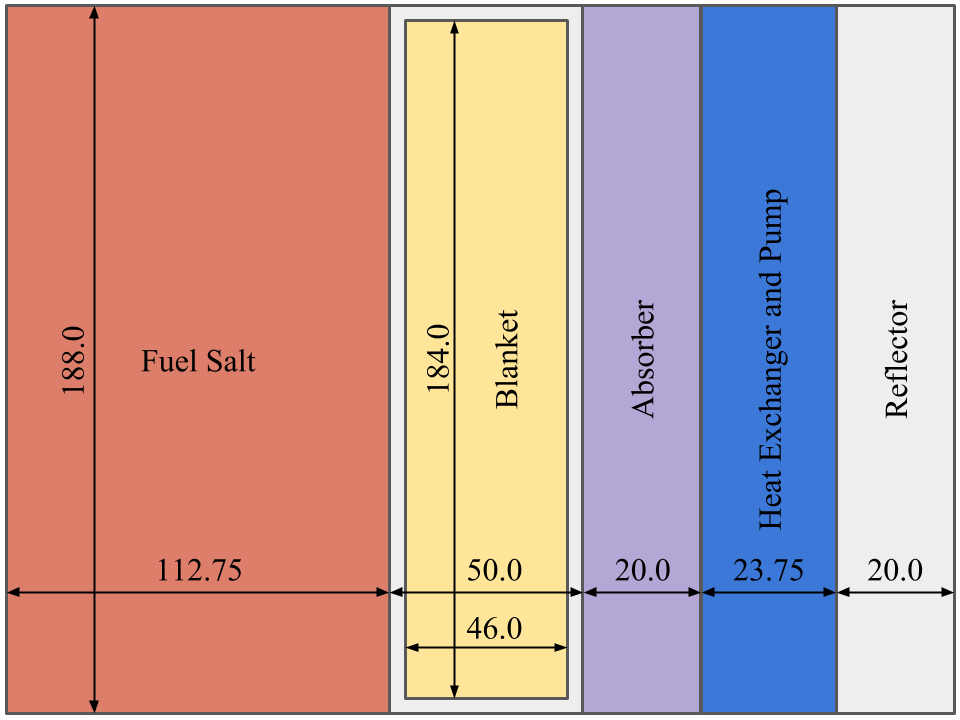
\includegraphics[width=0.47\textwidth]{./figures/reference}
	\captionsetup{justification=centering}
	\caption{Cross-section of the 2D axisymmetric model used in SERPENT.
	Derived from the \gls{MSFR} reference model
	\cite{pettersen_coupled_2016}. Figure is not drawn to scale. All dimensions
	are in cm.}
	\label{fig:reference}
\end{figure} 

\subsection{Moltres Code}

	This subsection provides the theoretical background for the coupled
	neutronics/thermal-hydraulics physics implemented in Moltres.
	
	Moltres is an application code developed in the \gls{MOOSE} framework
	\cite{gaston_moose:_2009}. \gls{MOOSE} application codes solve non-linear
	problems through the discretization of \glspl{PDE} on an adaptive coarse
	meshing scheme provided by LibMesh \cite{kirk_libmesh:_2006} and PetSc
	\cite{satish_balay_petsc_2015}. Individual terms of \glspl{PDE} that define
	the physics involved in a system are represented in \gls{MOOSE} (and its
	applications) by kernels. For example, the various terms in the neutron
	diffusion equation such as the diffusion term, time evolution term, etc.
	all have a corresponding physics kernel defined in Moltres. Boundary
	conditions are also handled in a similar fashion. Moltres can solve for an
	arbitrary number of neutronics groups as long as the relevant group
	constants are provided in a compatible text format.

	As mentioned in the previous Moltres study
	\cite{lindsay_introduction_2018}, the neutronics in Moltres is described by
	the time-independent multi-group neutron diffusion equation as shown in
	Equation \ref{eq1}:
%
\begin{align}
	\frac{1}{v_g} &\frac{\partial \phi_g}{\partial t} - \nabla \cdot D_g \nabla
	\phi_g + \Sigma^r_g \phi_g \nonumber \\ 
	&= \sum^G_{g \neq g'} \Sigma^s_{g' \rightarrow g} \phi_{g'} + \chi^p_g
	\sum^G_{g'=1} (1-\beta) \nu \Sigma^f_{g'} \phi_{g'} + \chi^d_g \sum^I_i
	\lambda_i C_i, \label{eq1}
\end{align}
%
	where
{\small
\begin{align*}
	v_g &= \text{average speed of neutrons in group }g \\
	\phi_g &= \text{flux of neutrons in group }g \\
	t &= \text{time} \\
	D_g &= \text{diffusion coefficient of neutrons in group }g \\
	\Sigma^r_g &= \text{macroscopic cross-section for removal of neutrons} 
	\nonumber \\
	&\text{from group }g
\end{align*}
%
\begin{align*}
	\Sigma^s_{g' \rightarrow g} &= \text{macroscopic cross-section of
	scattering from }g' \text{ to }g \\
	\chi^p_g &= \text{prompt fission spectrum neutrons in group }g \\
	G &= \text{number of discrete neutron groups, }g \\
	\nu &= \text{average number of neutrons produced per fission} \\
	\Sigma^f_{g} &= \text{macroscopic fission cross-section} \nonumber \\
	&\text{for neutron in group }g \\
	\chi^d_g &= \text{delayed fission spectrum neutrons in group }g \\
	I &= \text{number of delayed neutron precursor groups} \\
	\beta &= \text{delayed neutron fraction} \\
	\lambda_i &= \text{average decay constant of delayed neutron} \nonumber \\
	&\text{precursors in precursor group }i \\
	C_i &= \text{concentration of delayed neutron precursors} \nonumber \\
	&\text{in precursor group }i .
\end{align*}
}

	The \glspl{DNP} are governed by the following equation:
%
\begin{align}
	\frac{\partial C_i}{\partial t} = \sum^G_{g'=1} \beta_i \nu \Sigma^f_{g'}
	\phi_{g'} - \lambda_i C_i - \frac{\partial}{\partial z} u C_i. \label{eq2}
\end{align}

	Lastly, the governing equation for temperature in the molten salt is given
	as:
%
\begin{align}
	\rho c_{p} \frac{\partial T}{\partial t} + \nabla \cdot \big( \rho
	c_{p} \overrightarrow{u} \cdot T - k \nabla T \big) = Q_s - Q_{hx},
	\label{eq3}
\end{align}
%
	where
{\small
\begin{align*}
	\rho &= \text{density of molten salt} \\
	c_{p} &= \text{specific heat capacity of molten salt} \\
	T &= \text{temperature of molten salt} \\
	\overrightarrow{u} &= \text{velocity of molten salt} \\
	k &= \text{thermal conductivity of molten salt} \\
	Q_{hx} &= \text{heat sink},
\end{align*}
}
	and the source term $Q_s$ is given as:
%
\begin{align}
Q_s = \sum^G_{g=1} \epsilon_g \Sigma_g^f \phi_g. \label{eq4}
\end{align}
%
\begin{figure}[h] 
	\centering
	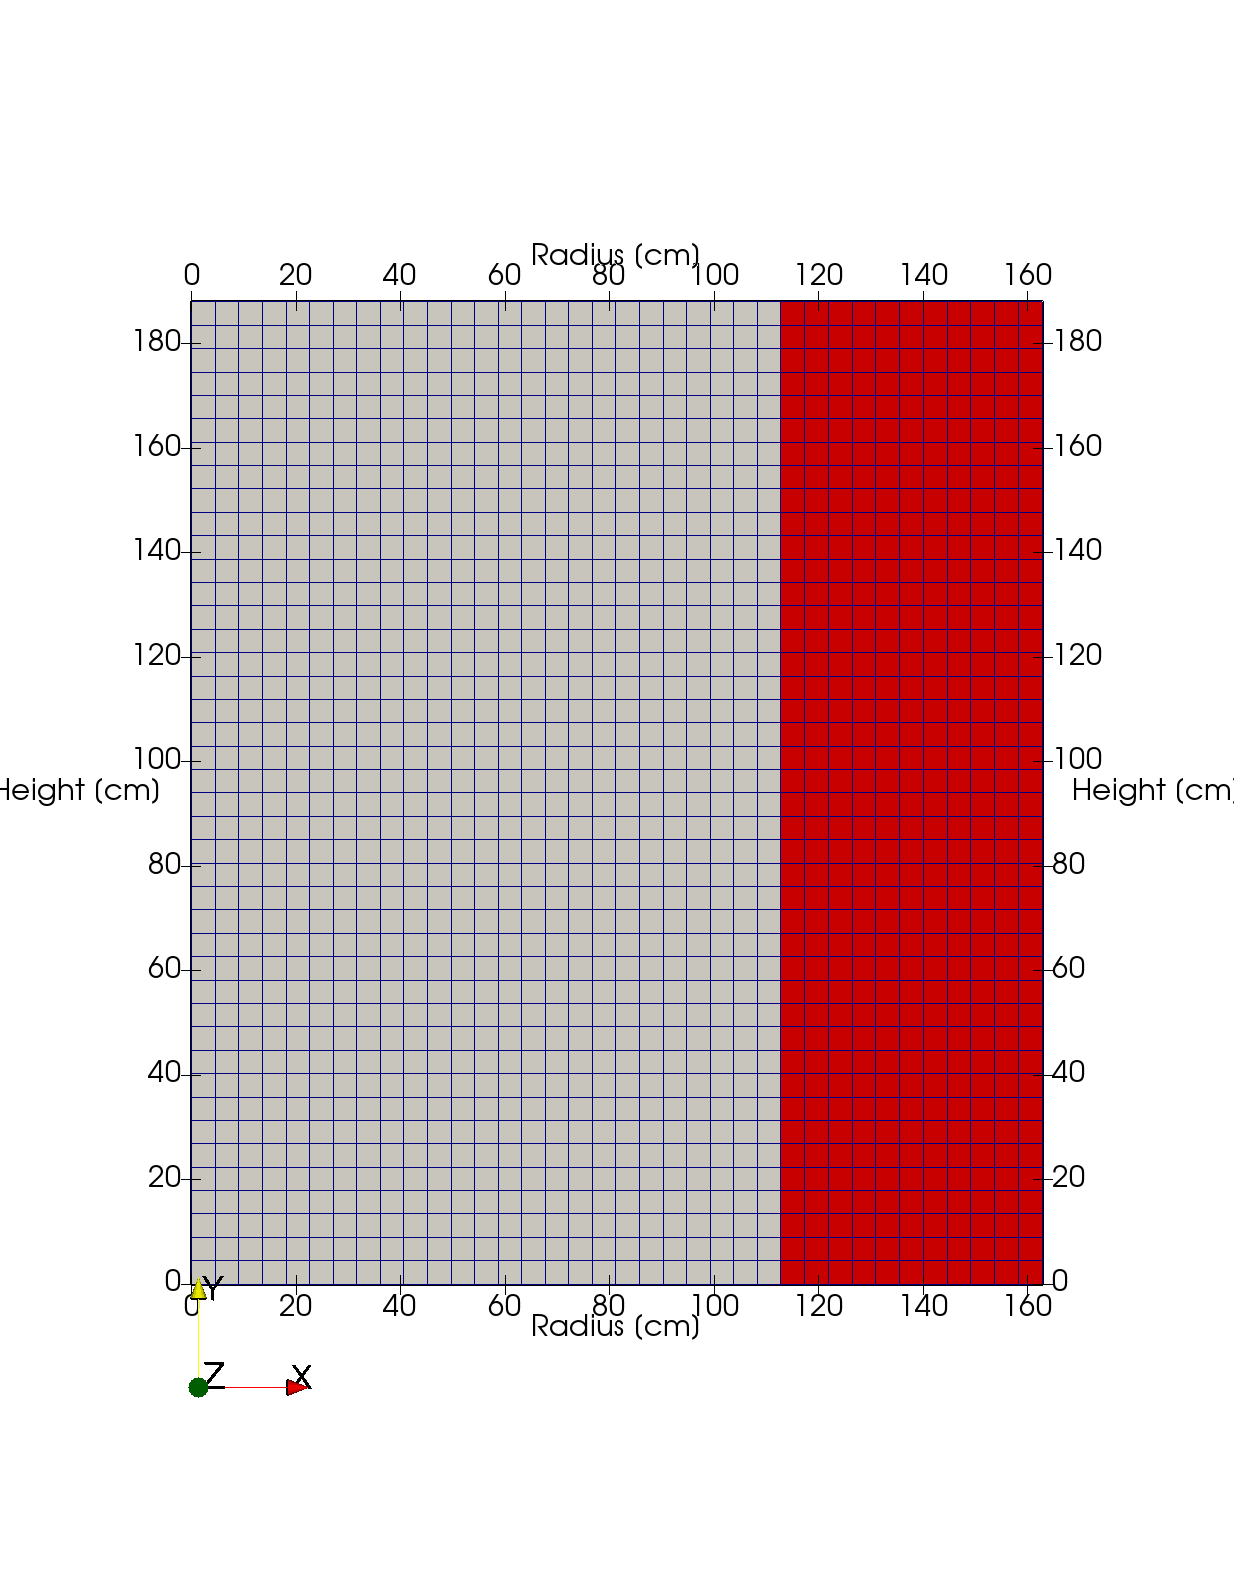
\includegraphics[width=0.45\textwidth]{./figures/mesh}
	\captionsetup{justification=centering}
	\caption{Mesh of the 2D axisymmetric model used in Moltres.
	The grey and red regions represent the fuel and blanket salt respectively.}
	\label{fig:mesh}
\end{figure} 

\section{Steady State Neutron Flux \\and Temperature Distribution}

	We first ran Moltres in steady-state solver mode to generate the six-group
	neutron flux distribution at a temperature of 973 K with the start-up fuel
	composition. This
	is verified against the six-group flux generated directly from SERPENT
	after collapsing the fine-group flux.
	Figure \ref{fig:ntflux} shows the neutron flux
	distributions from SERPENT and Moltres, with precursor drift disabled for
	code verification. There is very good agreement between the six group
	flux distributions from SERPENT and Moltres.
	
	Next, the \gls{MSFR} Moltres simulations were
	run in transient mode, with adaptive time-stepping and an
	initial, uniform neutron flux of $10^{14}$
	cm$^{-2}$ s$^{-1}$ and an initial temperature of 923 K throughout the
	fuel and blanket regions, for the start-up, early-life, and equilibrium
	fuel compositions. The simulations reached steady state after 100 s, as the
	volume-integrated neutron flux values varied by less than 0.001\% over the
	previous ten seconds. The computational time for each case averages at 30
	minutes when run on four processing units on a workstation.

\begin{table}[b]
	\centering
	\captionsetup{justification=centering}
	\caption{Average fuel inlet temperature.}
	\begin{tabular}{lS}
		\hline
		{Composition} & {Inlet temperature [K]}\\
		\hline
		Start-up & 964.85\\
		Early-life & 925.11\\
		Equilibrium & 916.85\\
		\hline
	\end{tabular}
	\label{table:inlet}
	\centering
	\captionsetup{justification=centering}
	\caption{Average fuel outlet temperature.}
	\begin{tabular}{lS}
		\hline
		{Composition} & {Outlet temperature [K]}\\
		\hline
		Start-up & 1067.40\\
		Early-life & 1025.39\\
		Equilibrium & 1016.67\\
		\hline
	\end{tabular}
	\label{table:outlet}
\end{table}	
%
\begin{figure}[htbp] 
	\centering
	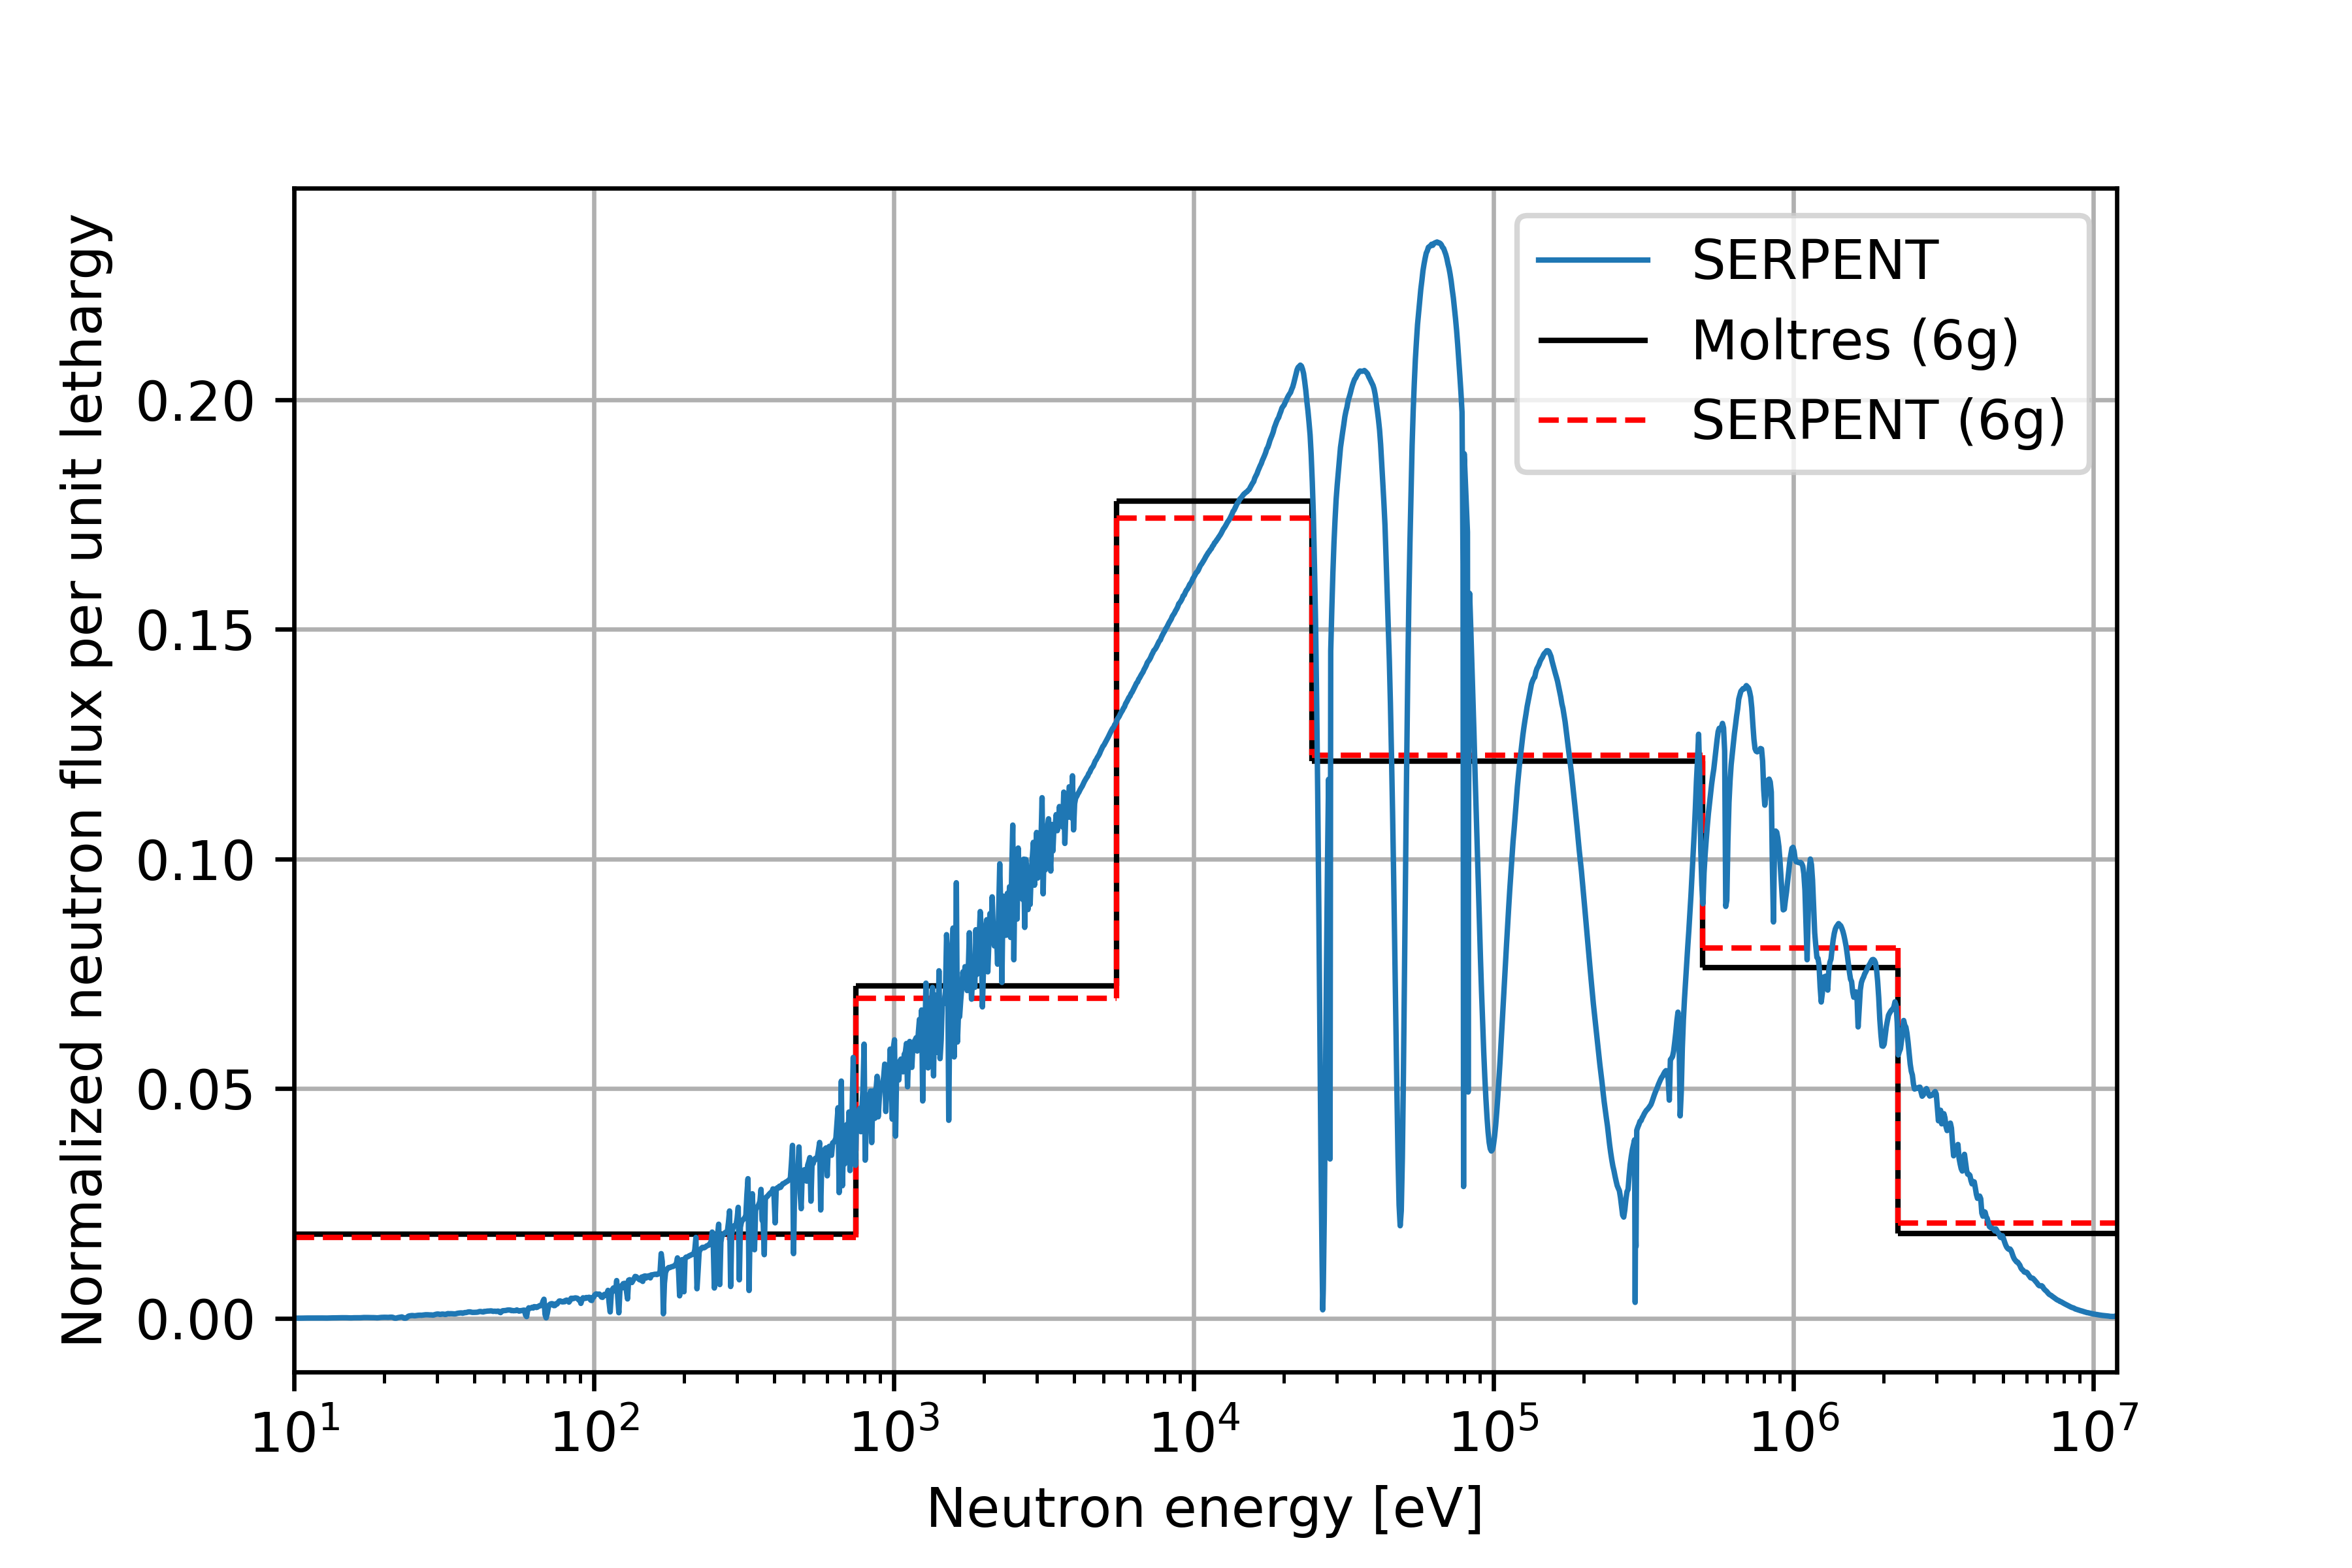
\includegraphics[width=.48\textwidth]{./figures/nt-spec}
	\captionsetup{justification=centering}
	\caption{Fine-group and six-group neutron flux\\ distributions from SERPENT
	and Moltres.}
	\label{fig:ntflux}
	\centering
	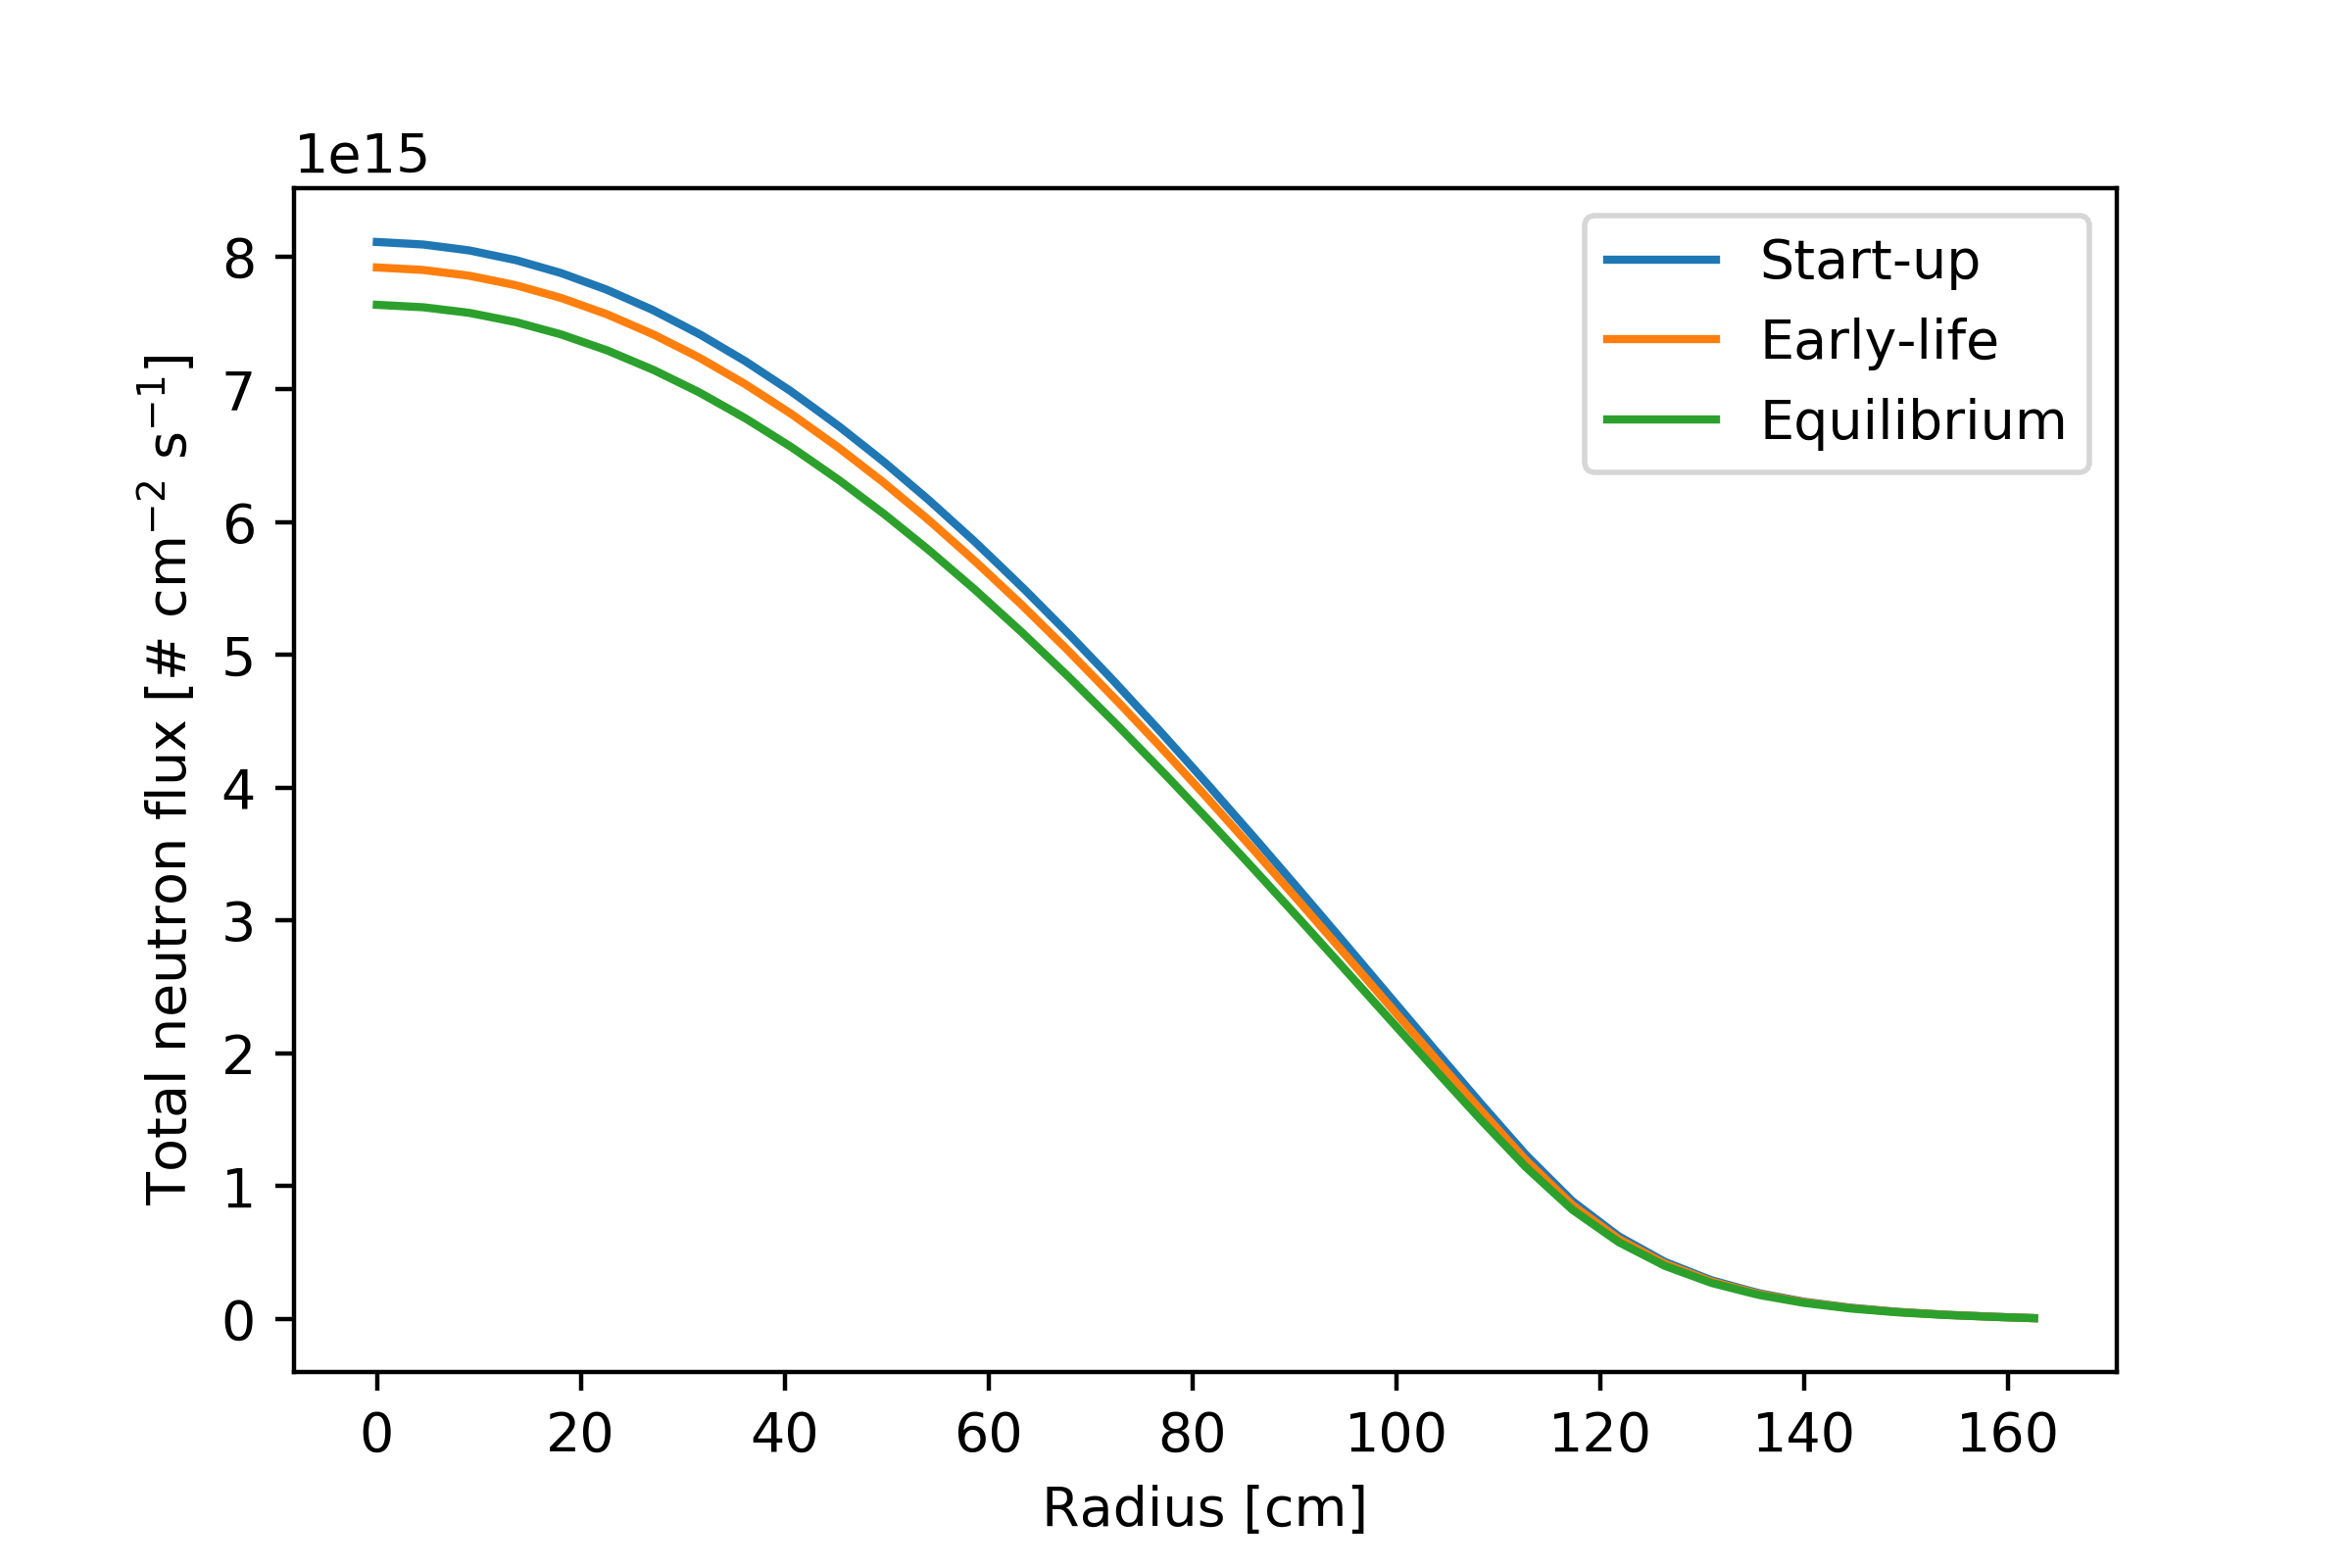
\includegraphics[width=.48\textwidth]{./figures/totalflux}
	\captionsetup{justification=centering}
	\caption{Total radial neutron flux at reactor half-height, for start-up,
	early-life, and equilibrium fuel compositions at steady state.}
	\label{fig:totalflux}
	\centering
	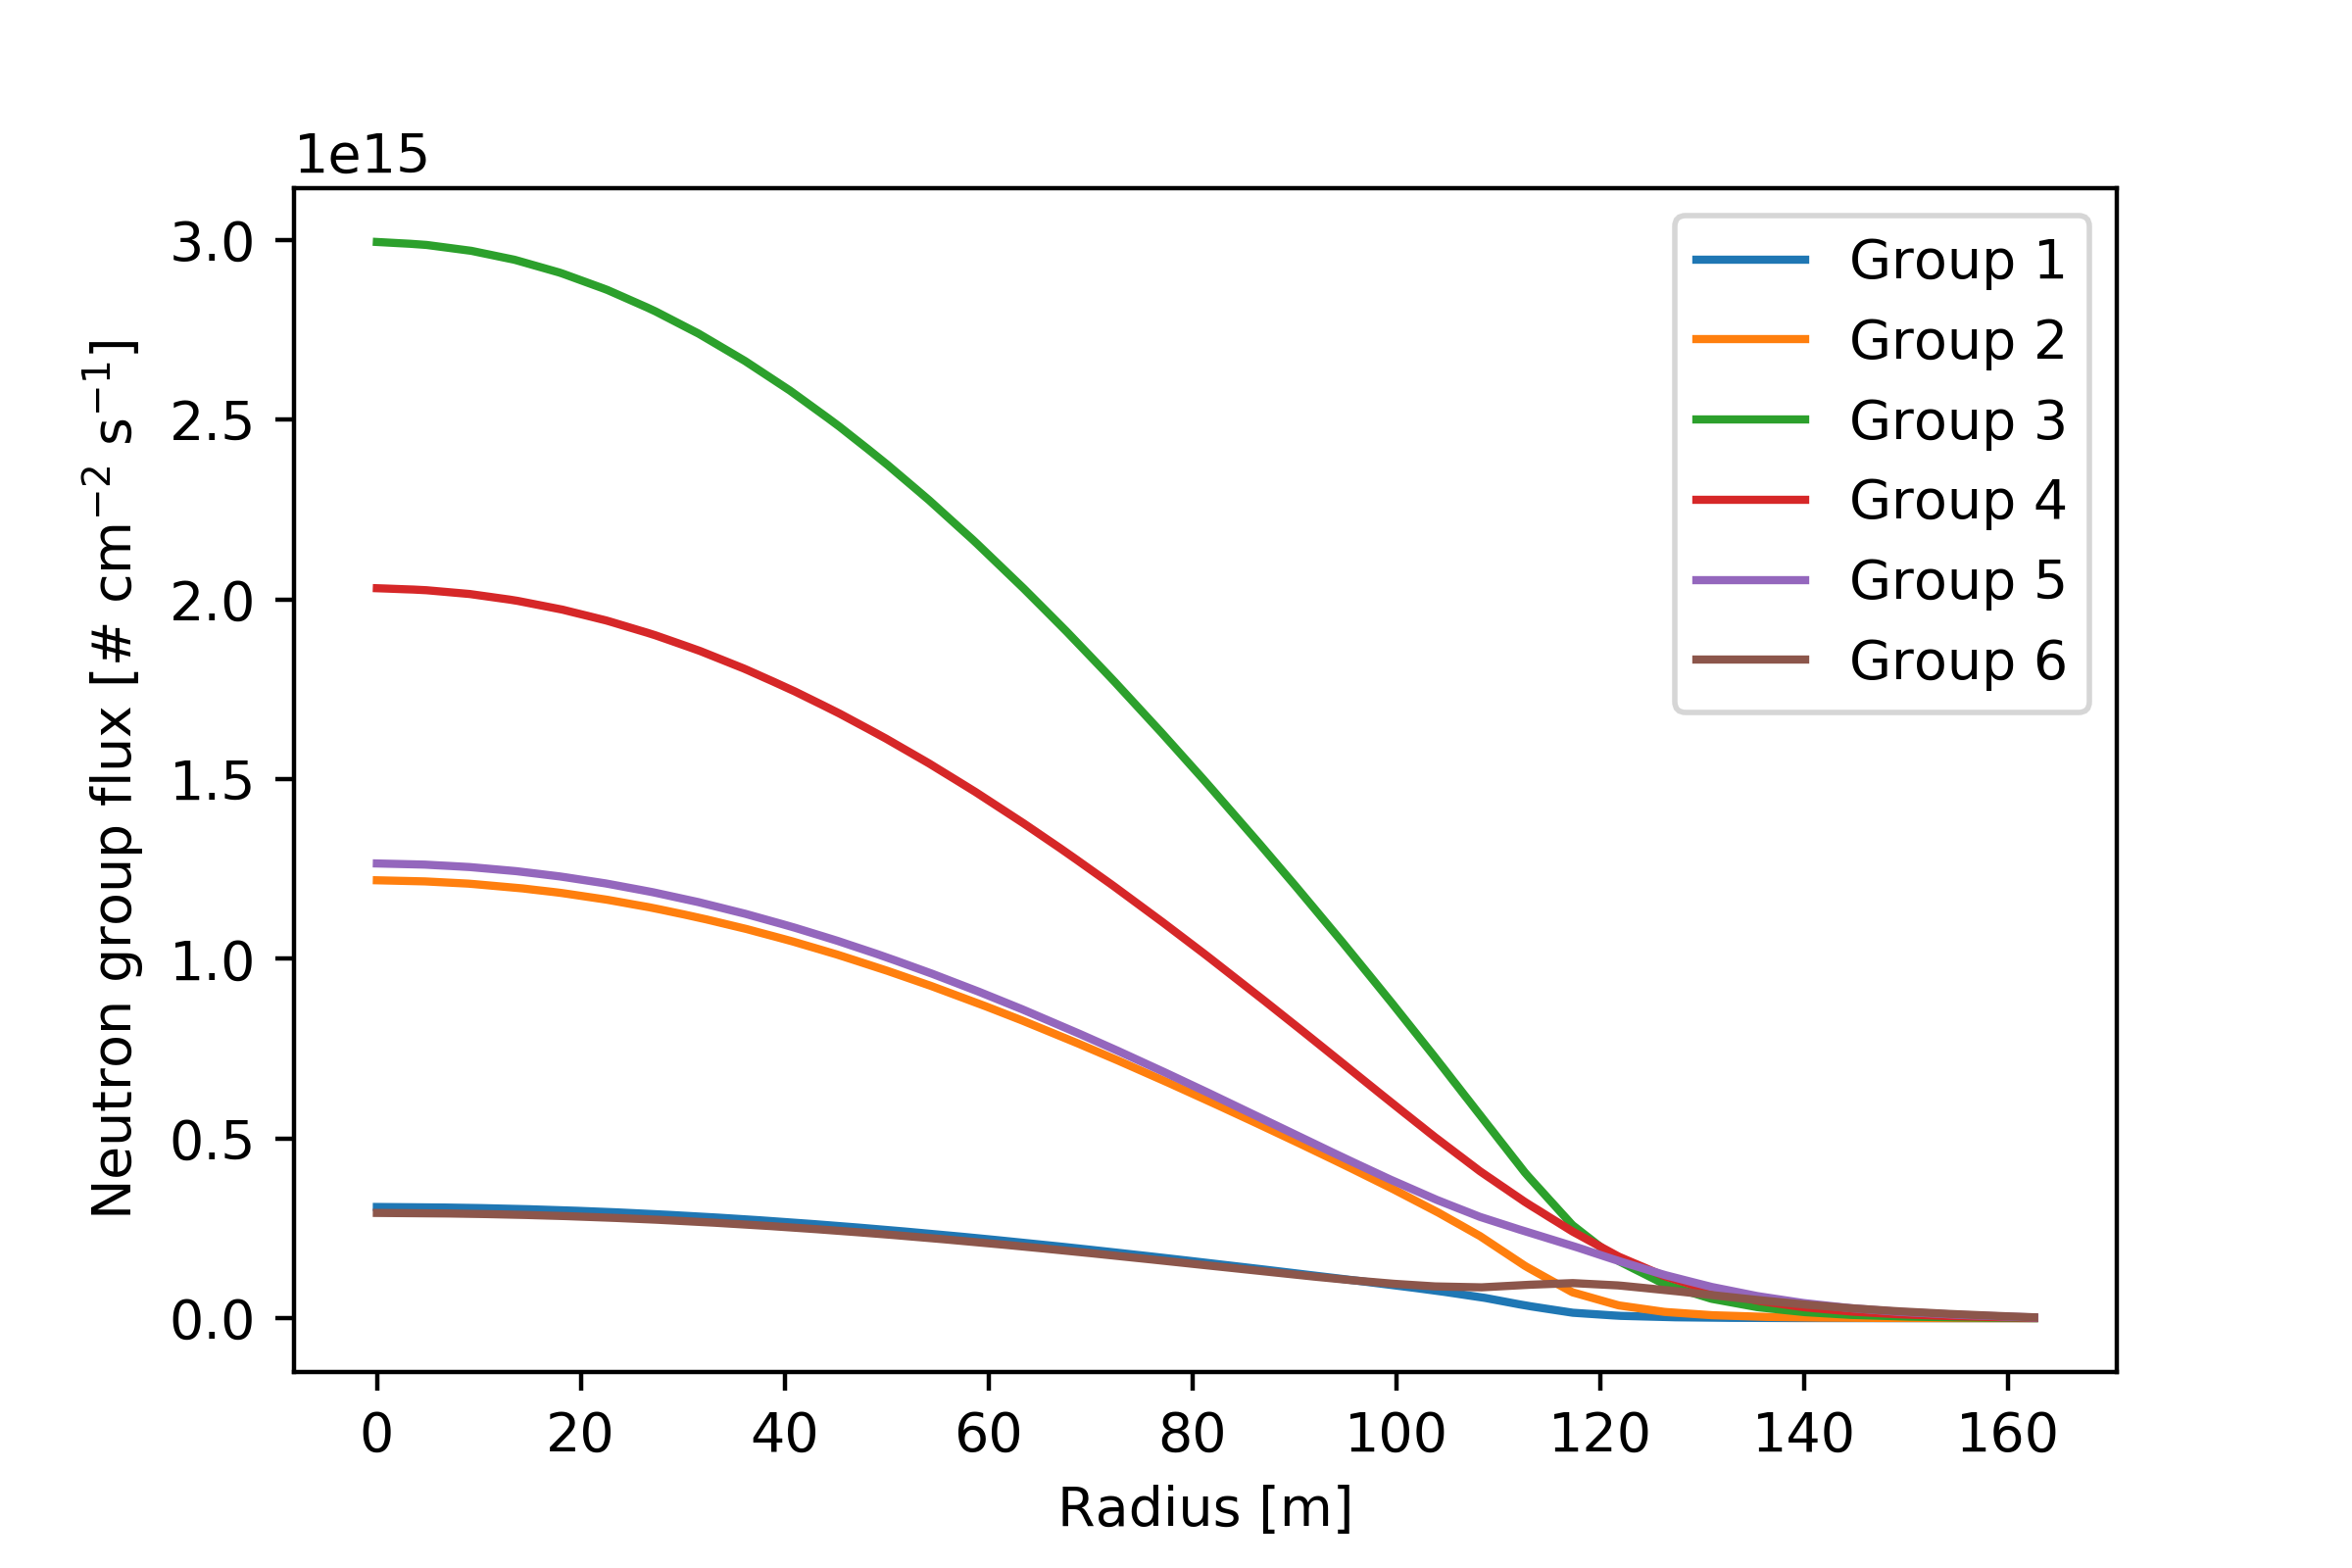
\includegraphics[width=.48\textwidth]{./figures/stflux}
	\captionsetup{justification=centering}
	\caption{Neutron group fluxes at reactor half-height, for start-up
	fuel composition at steady state.}
	\label{fig:stflux}
\end{figure}
%
\begin{figure*}[htbp]%
\centering
\begin{subfigure}{1\columnwidth}
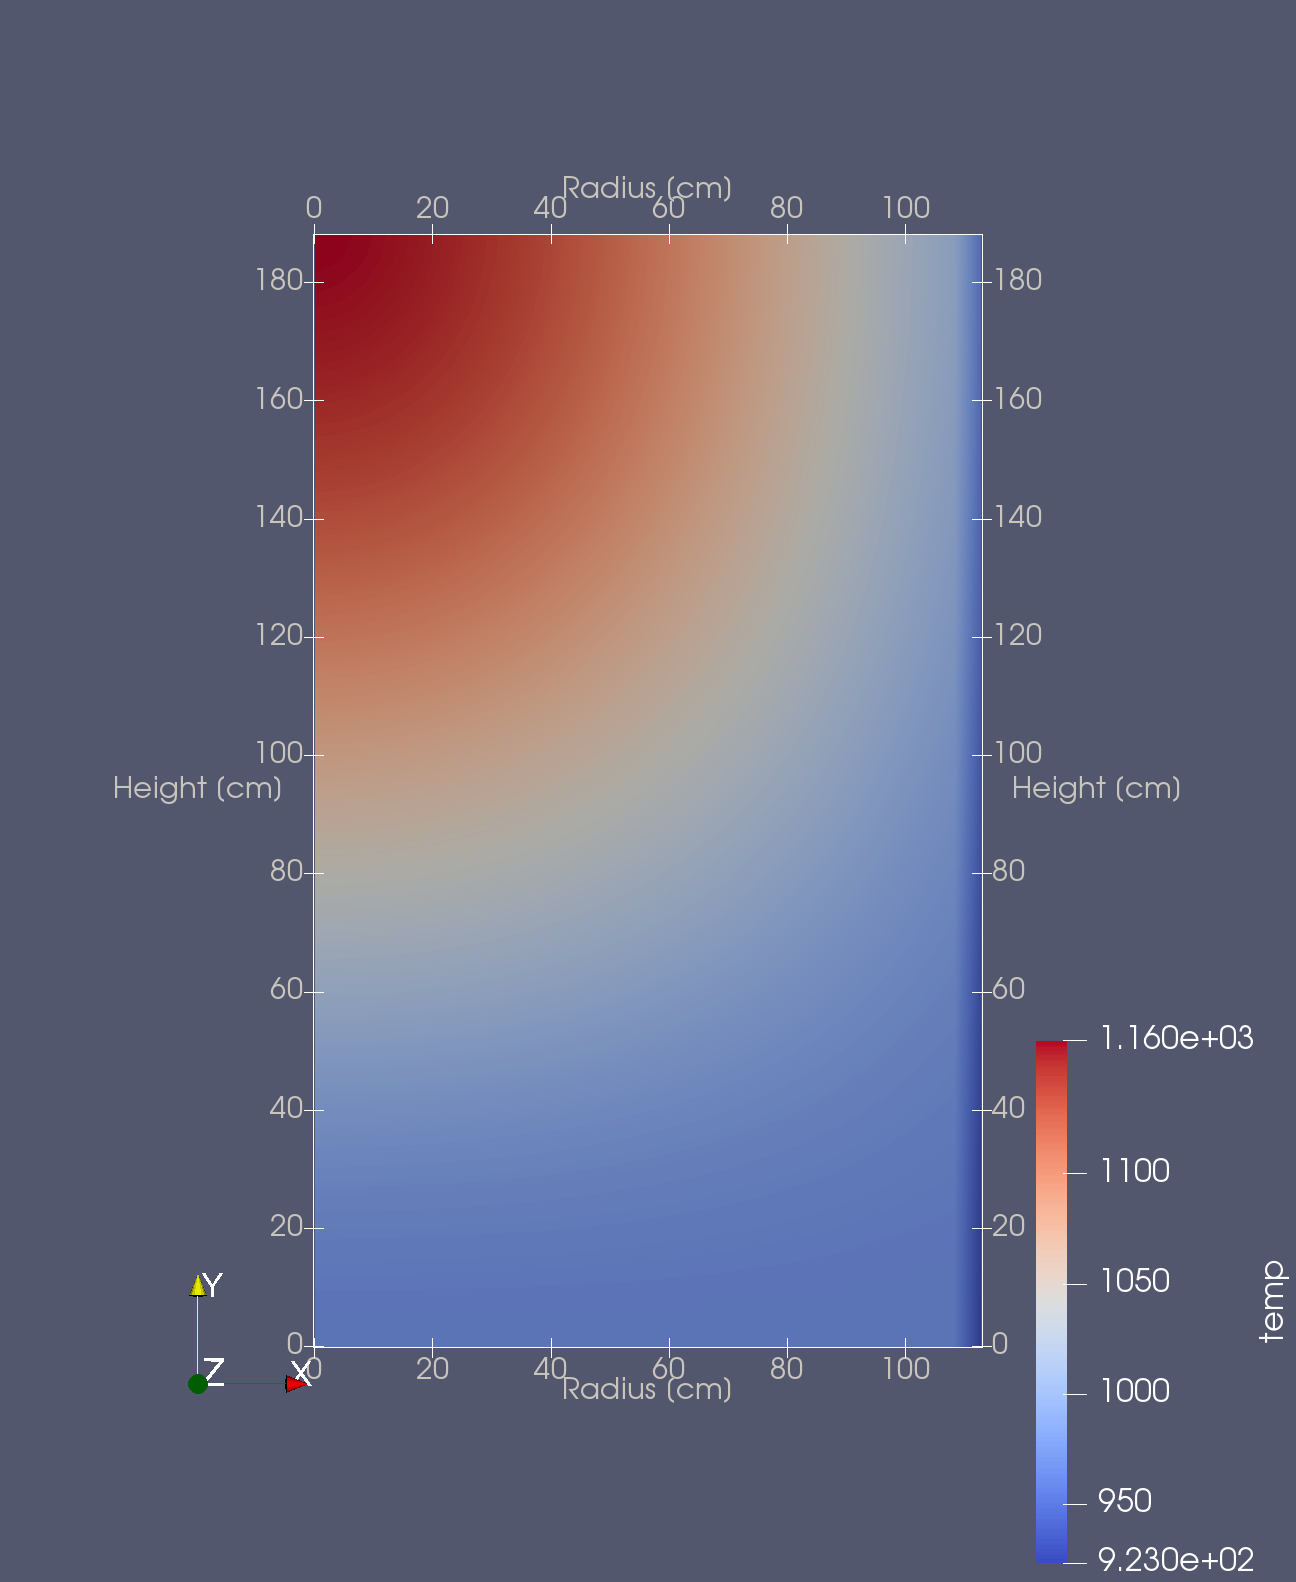
\includegraphics[width=\columnwidth]{./figures/sttemp}%
\end{subfigure}\hfill%
\begin{subfigure}{1\columnwidth}
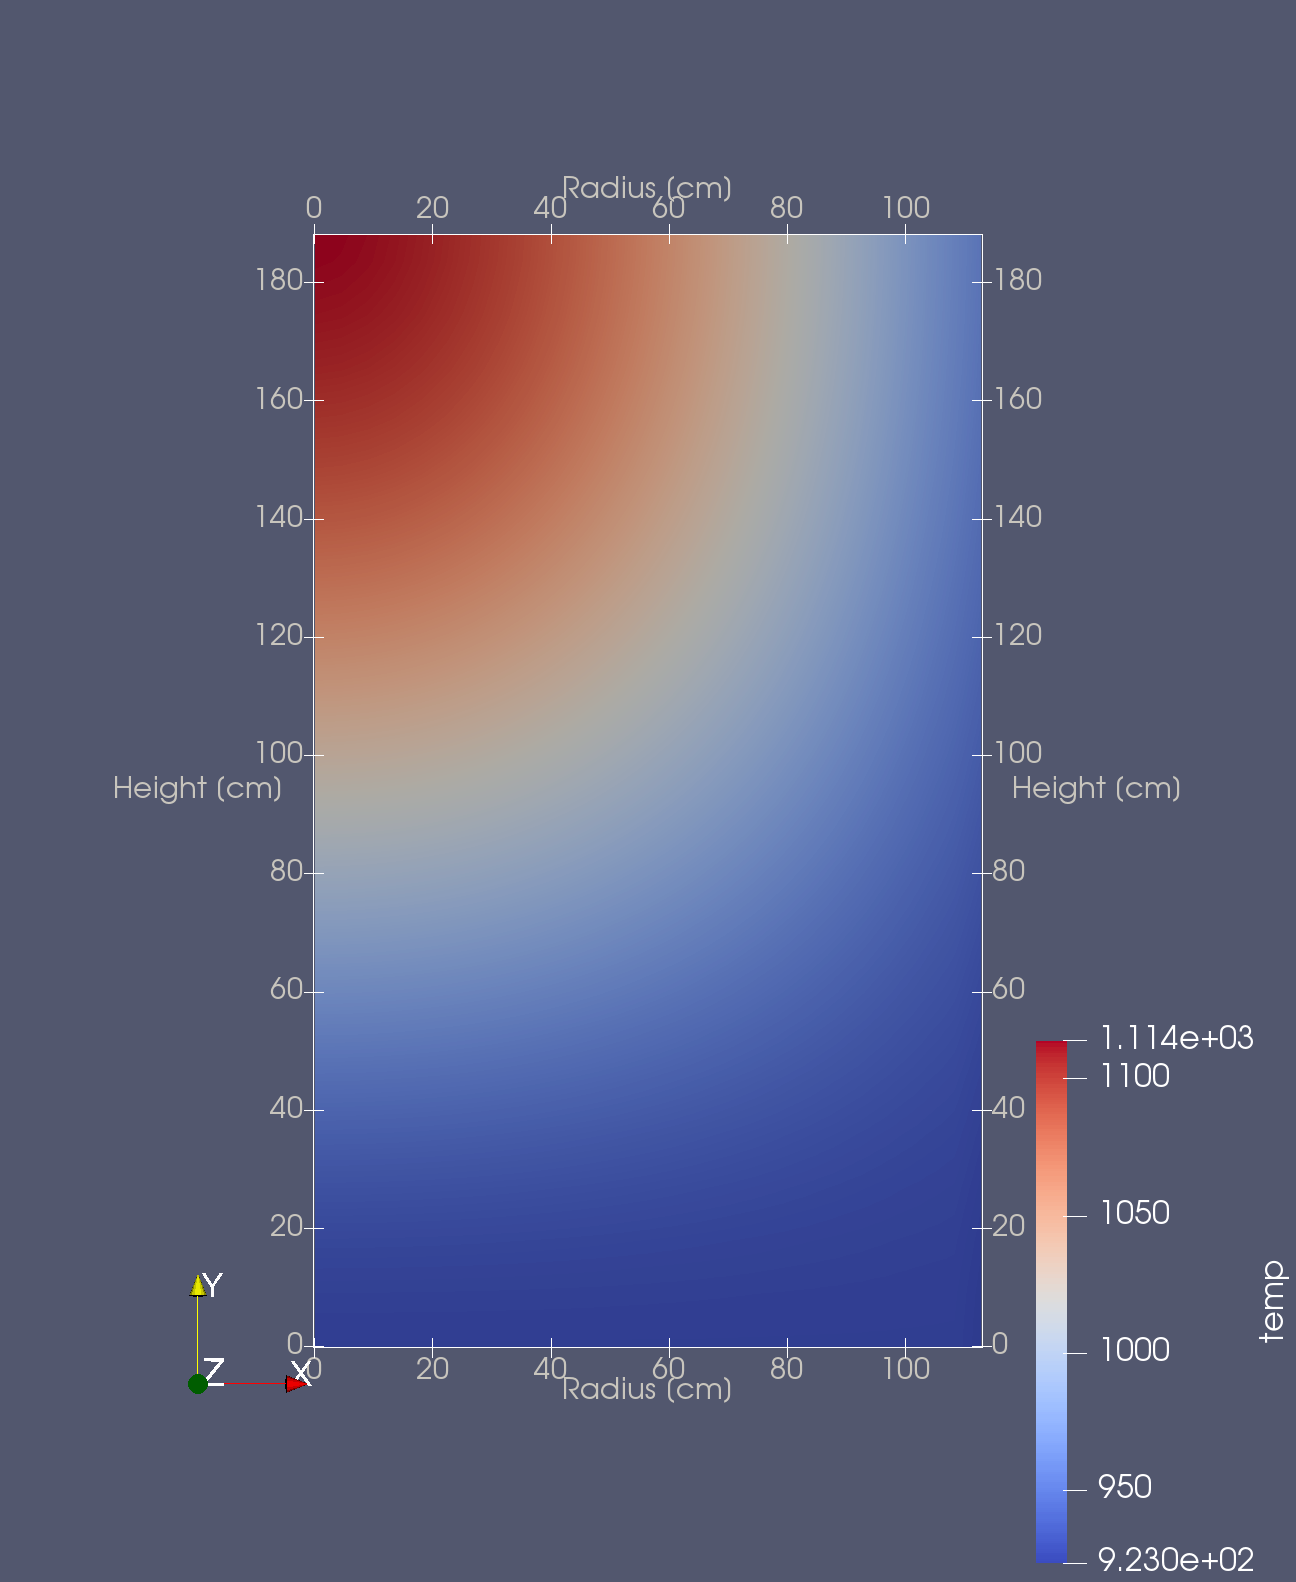
\includegraphics[width=\columnwidth]{./figures/eltemp}%
\end{subfigure}\hfill\\
\bigskip
\centering
\begin{subfigure}{1\columnwidth}
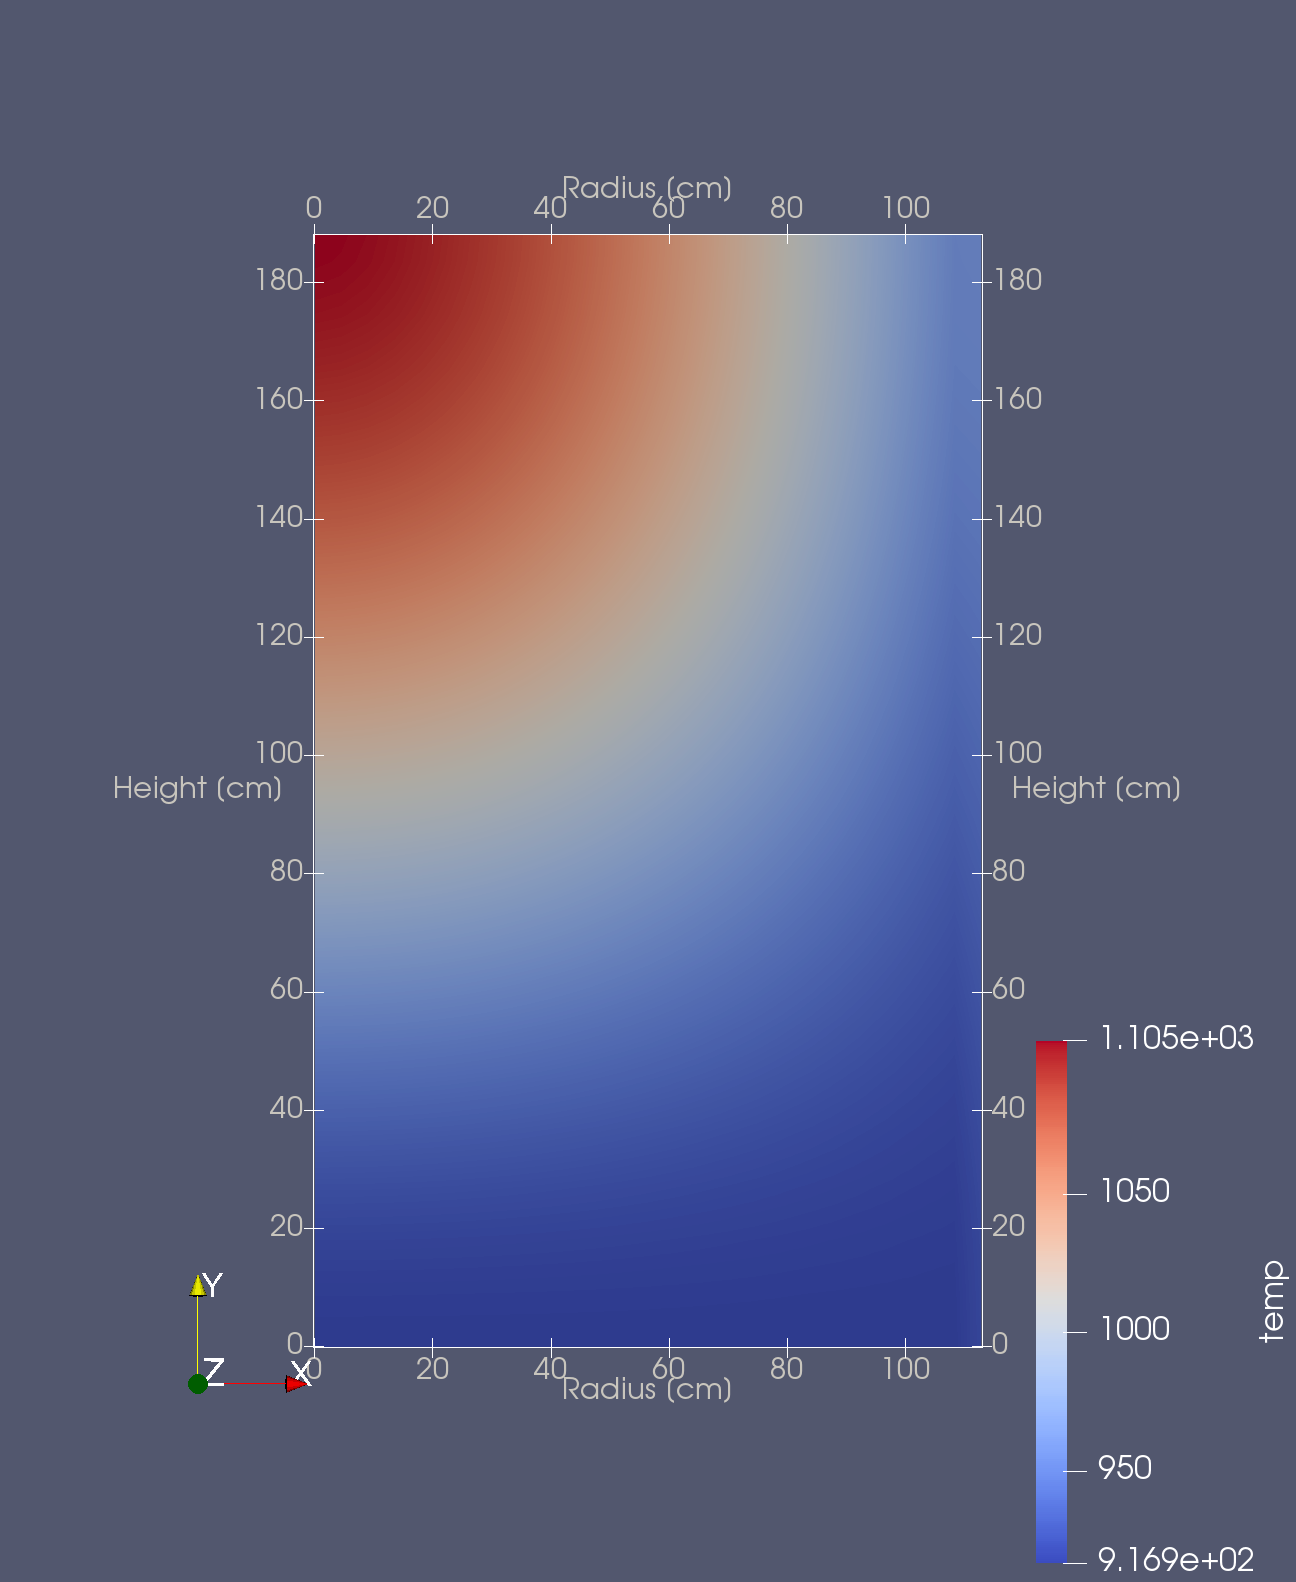
\includegraphics[width=\columnwidth]{./figures/eqtemp}%
\label{subfigc}%
\end{subfigure}%
\captionsetup{justification=centering}
\caption{Temperature distributions within the fuel salt region, for start-up
(top left), early-life (top right), and equilibrium (bottom) fuel compositions
at steady state. The height and radius are in the Y and X directions
respectively.}
\label{fig:temp}
\end{figure*}
	
	Figure \ref{fig:totalflux} shows the total radial neutron flux at reactor
	half-height, with the three fuel compositions at steady state. 
	The peak neutron flux value is highest for the start-up composition,
	followed by the early-life and equilibrium compositions. All three values
	are slightly lower than the peak value of approximately
	$8.6 \times 10^{15}$ cm$^{-2}$ s$^{-1}$ reported by Fiorina et al.
	\cite{fiorina_investigation_2013}. This may be due to the truncation of
	the top and bottom fuel regions of the core for the model used here.
	The vacuum boundary conditions were imposed closer to the center and
	resulted in a lower peak value. Figure \ref{fig:stflux} shows the six
	neutron group fluxes for the start-up fuel composition.
	
	Heat transfer is dominated by advection as is observed by the temperature
	distributions in Figure \ref{fig:temp}. Given that flux is the highest
	at the center of the core, most of the heat is produced there. The upward
	flow pushes the temperature peak up to the outlet boundary. Tables
	\ref{table:inlet} and \ref{table:outlet} show the average
	fuel inlet and outlet temperatures for the three cases.

	The average outlet temperatures for all three compositions are close to
	the \gls{MSFR} outlet temperature specification of 1023 K. Due to having a
	Reynolds number, significant
	mixing and heat transfer is expected in the fuel salt as it flows
	out of the core and through the outer loop. However, the center of the top
	reflector region is exposed to dangerously high peak temperatures
	of greater than 1100 K in all three cases as observed in Figure
	\ref{fig:temp}. In addition, higher temperatures
	are expected during dangerous accident scenarios.
	
	In actuality, the peak temperatures are likely to be lower than the values
	seen in Figure \ref{fig:temp} because of turbulent mixing. In choosing a
	uniform velocity profile, we have also implied that flow is laminar, which
	is a weak assumption given the high Reynolds number of molten salt flow in
	the \gls{MSFR}. Turbulent temperature mixing could potentially be
	approximated by
	incorporating it into the conduction term as turbulent diffusion.
	
	The uniform velocity approximation in our models also resulted in a
	significantly different spatial temperature distribution shape as compared
	to
	the results by Fiorina et al. \cite{fiorina_modelling_2014} and Pettersen
	\cite{pettersen_coupled_2016}. Their models feature significant flow
	stagnation in the fuel salt
	near the blanket tank. This causes their temperatures distributions to peak
	near the blanket
	tank as opposed to the center of the core as seen in Figure \ref{fig:temp}.
	However, improved models of the \gls{MSFR}, as shown by Aufiero et al.
	\cite{aufiero_development_2014}, have temperature distributions closer to
	the results in this paper through curved walls that optimize salt flow.
	
	Total power, as defined by Eq. \ref{eq4}, at steady state is approximately
	2 GW. This
	is 1 GW less than the rated 3 GW of the \gls{MSFR}. This may be mainly due
	to the erroneous uniform velocity profile imposed in the core. From
	fluid dynamics, velocity along the central axis of the core should be
	higher than the velocity at the periphral areas near the blanket tank.
	The higher velocity at the center results in higher advective heat transfer
	away from the center of the core and cools the active region. This should
	result in an increase in neutron flux from the strong negative
	temperature reactivity feedback, and thus higher heat generation. The
	truncation of the top and bottom fuel salt region is also a factor for
	the lower than expected heat production.
	
	Comparing the three different fuel compositions, the \gls{MSFR} operates at
	the highest temperatures with the start-up fuel composition, followed by
	the early-life, and the equilibrium compositions. This may be due to the
	generation of $^{233}$Pa as an intermediate for $^{233}$U breeding as
	mentioned by Rykhlevskii et al. \cite{rykhlevskii_fuel_2019} in their fuel
	cycle analysis
	of the \gls{MSFR}; $^{233}$Pa is a precursor for the $^{234}$U neutron
	poison.
	
\begin{figure}[t] 
	\centering
	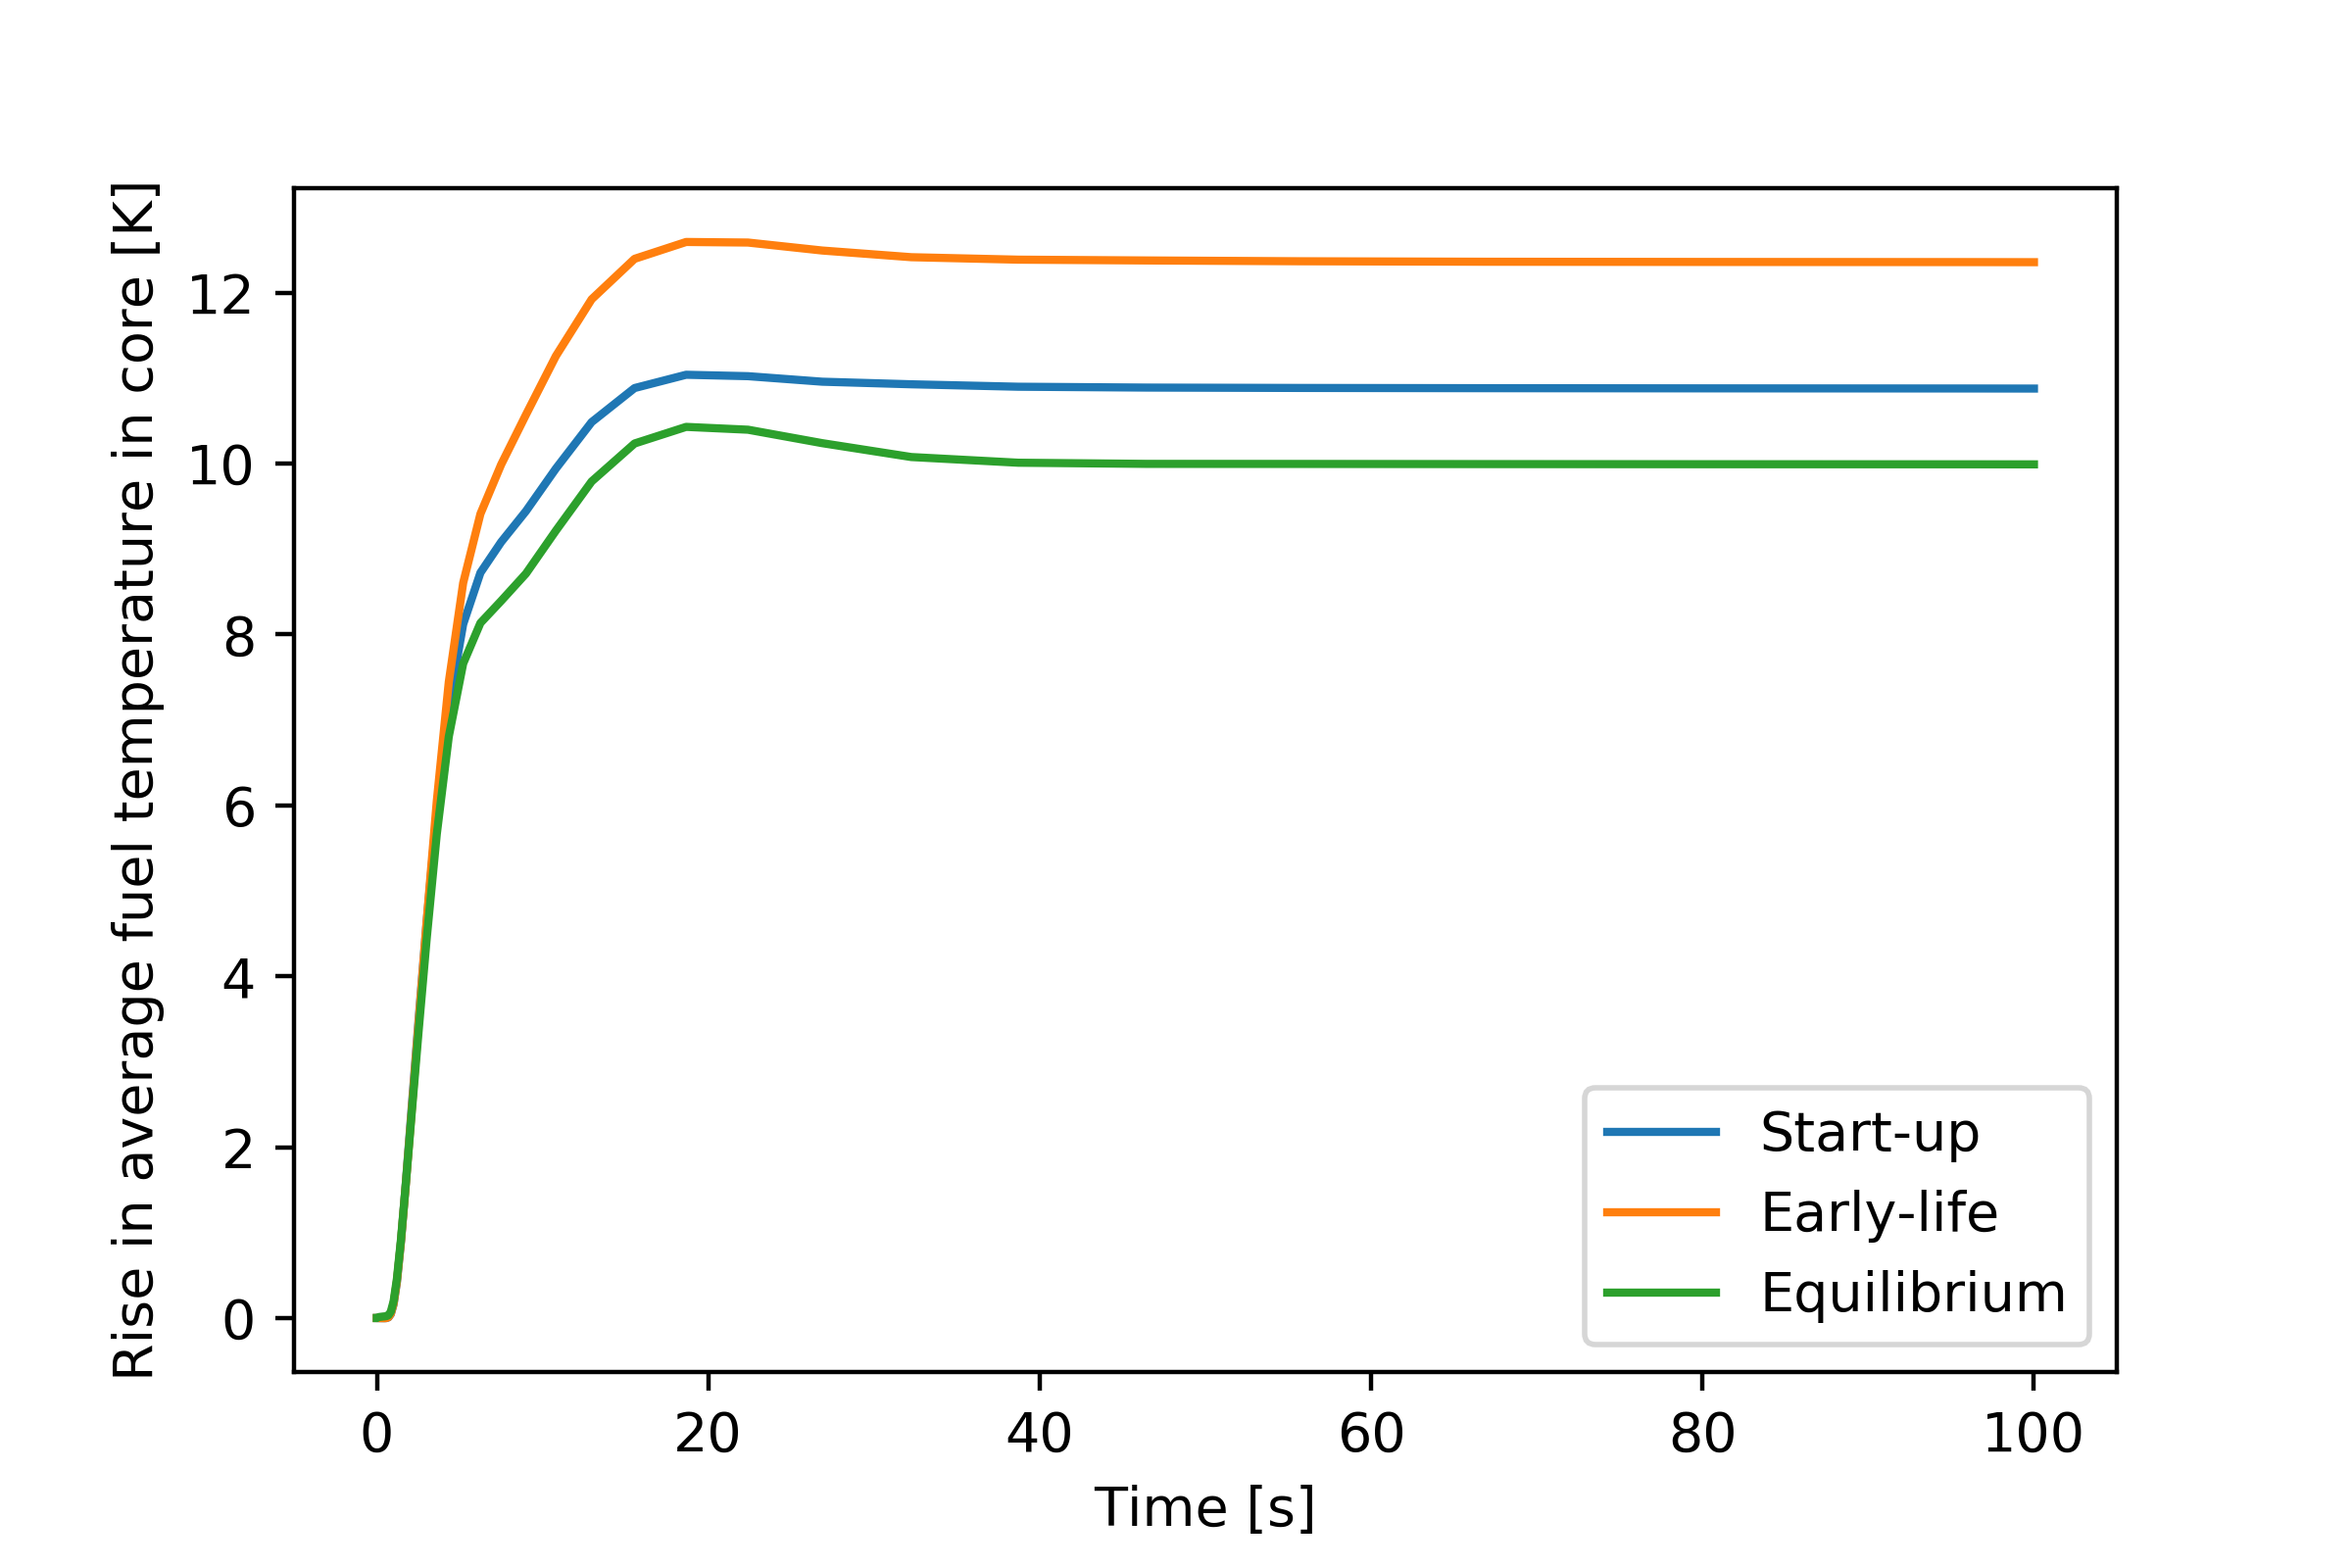
\includegraphics[width=.48\textwidth]{./figures/loscatemp}
	\captionsetup{justification=centering}
	\caption{Rise in average core fuel temperature for start-up, early-life,
	and equilibrium fuel compositions during \gls{ULOHS}.}
	\label{fig:loscatemp}
	\centering
	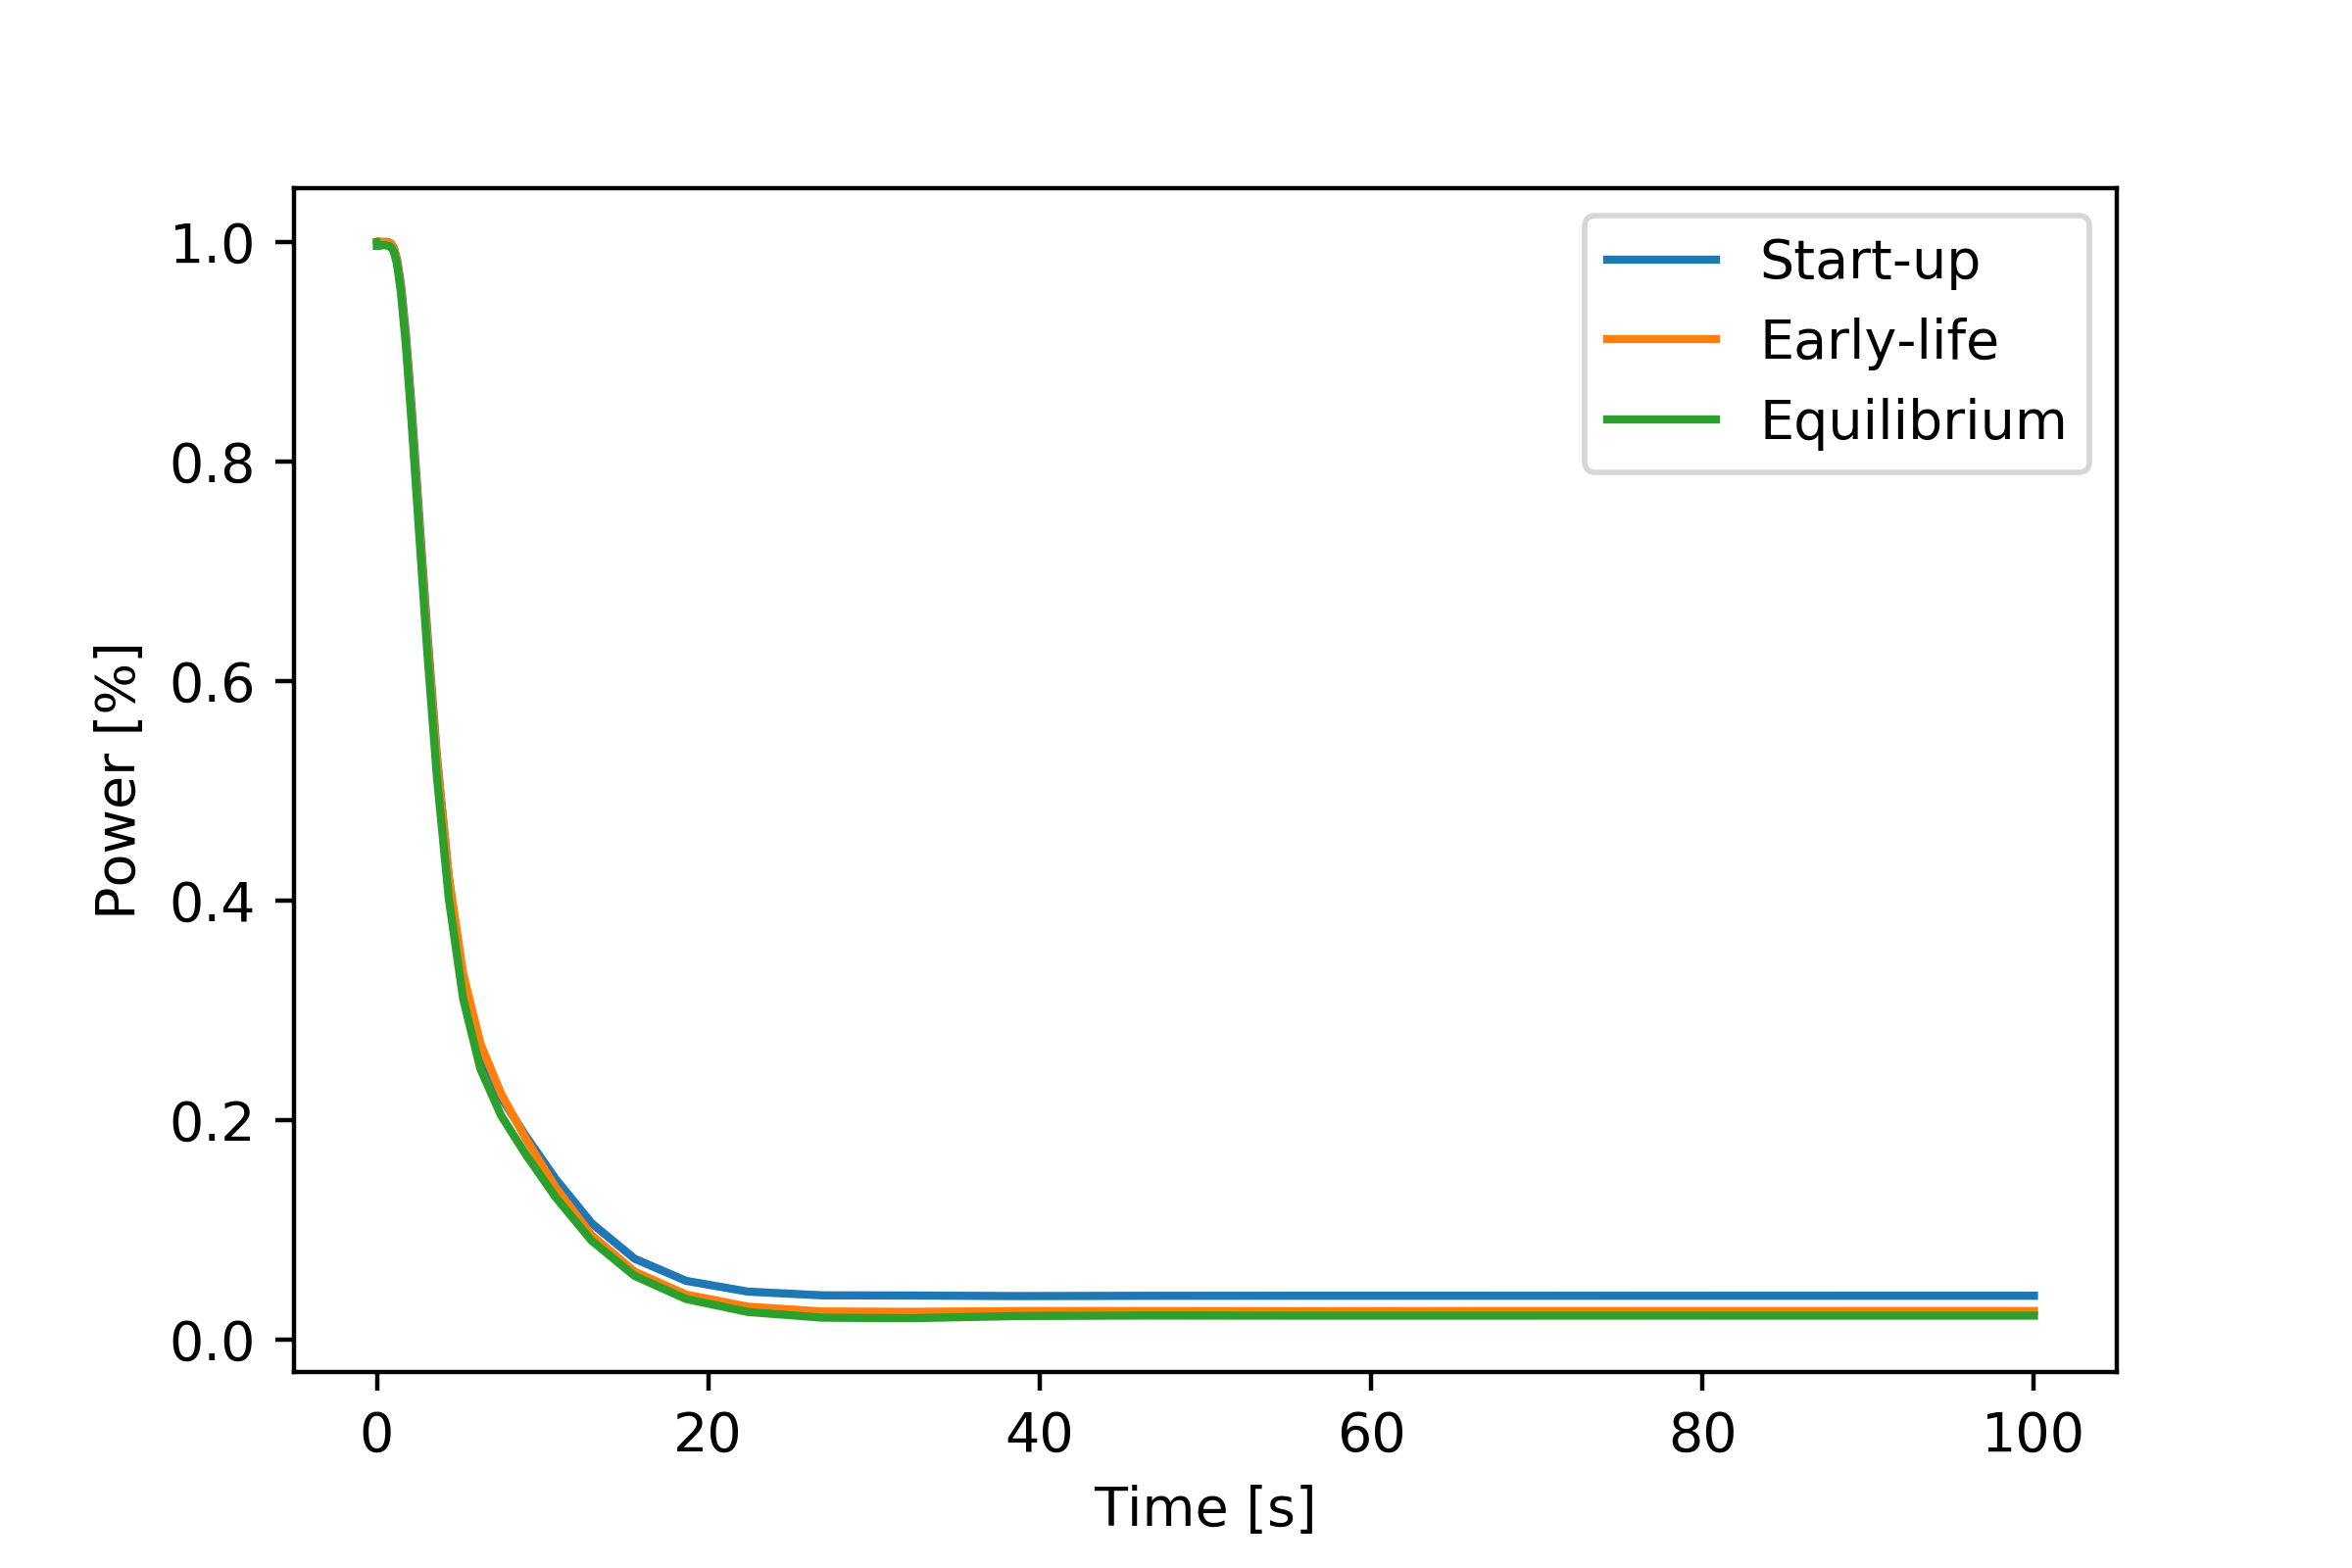
\includegraphics[width=.48\textwidth]{./figures/loscaheat}
	\captionsetup{justification=centering}
	\caption{Power generated, for start-up, early-life, and
	 equilibrium fuel compositions during \gls{ULOHS}.}
	\label{fig:loscaheat}
\end{figure} 

\section{Unprotected Loss of Heat Sink}

	\gls{ULOHS} may occur due to various causes of failure in the heat
	exchanger or secondary
	coolant loop such as secondary loop pump failure or loss of secondary
	coolant. While it is less likely in an \gls{MSFR} as it consists of 16
	separate coolant loops each with its own secondary cooling system, the
	potential consequences must still be studied.
	The loss of secondary cooling is simulated by exponentially decreasing
	the heat loss rate in the Moltres heat exchanger kernel with a time
	constant of 5 s.
	
	\gls{ULOHS} is expected to cause temperatures to increase,
	followed by a decrease in neutron flux and heat generation due to the
	strong negative temperature reactivity feedback. Eventually, the
	\gls{MSFR} should settle on a new steady state with a higher average
	temperature than the operating temperature. If the high temperature is
	sustained for a long period of time, it could lead to severe damage
	in the reactor, pipes, or other instruments.

	As observed in Figure \ref{fig:loscatemp}, the average fuel temperature
	starts rising approximately 0.7 s after initiation. The \gls{MSFR} reaches
	a new steady state approximately 10 K higher than the initial temperature
	after 30 s. While the transition time to reach the new steady state is in
	good agreement with results reported by
	Fiorina et al. \cite{fiorina_modelling_2014}, the temperature rise is much
	smaller than the 100 K increase reported by the same authors.
	Power generation falls by two orders of
	magnitude (Figure \ref{fig:loscaheat}),
	resulting in a negligible temperature difference between the
	inlets and outlets for all three fuel compositions. This could also be
	attributed to the relatively small total power of 2 GW discussed in the
	previous section, and the truncated \gls{MSFR} model.
	
	In comparing the three fuel compositions, an \gls{MSFR} loaded with
	start-up fuel composition is at a higher safety risk as it has higher
	temperatures under normal operating conditions and accident scenarios.

\section{Conclusion}

	In this study, we investigated the steady state, and transient behavior of
	the \gls{MSFR} during a \gls{ULOHS}
	using the coupled neutronics/thermal-hydraulics code Moltres. Moltres
	boasts relatively fast computational times due to a combination of
	parallelization, adaptive coarse meshing scheme and adaptive time-stepping.
	We verified the six-group neutron flux distribution at 973 K from Moltres
	against SERPENT. The total peak
	neutron flux at steady state agrees very closely with published results by
	Fiorina et al. \cite{fiorina_modelling_2014}.
	
	While the temperature
	distribution and total power have
	large discrepancies, we have accounted for the main sources of error:
	the erroneous uniform velocity profile and the reactor model truncation. We
	also observed that the \gls{MSFR} operates at a higher temperature with the
	start-up fuel composition than with the early-life and equilibrium
	compositions, due to the presence of $^{233}$Pa. The high peak temperatures 
	near the center of the top reflector are a potential safety risk. While
	this high temperatures could have been exacerbated by absence of turbulent
	diffusion implementation in Moltres, it warrants the need for further
	safety analysis.
	
	During a \gls{ULOHS}, the \gls{MSFR} core fuel salt temperatures rise by
	approximately 10 K after a transition time of 30 s. While this time
	duration is
	similar to published results, the temperature rise is relatively low
	compared to the 100 K rise reported by Fiorina et al.
	\cite{fiorina_modelling_2014} This discrepancy is also attributed to the
	same sources of error for the steady state results. Nonetheless, a
	temperature rise of
	this magnitude is relatively benign to reactor components, and makes
	a strong safety case for \glspl{MSR} due to their strong negative
	temperature feedback, with the exception of the central top reflector
	region discussed previously.
	
	Further development of the models is necessary to improve the accuracy
	and reliability of Moltres as a coupled neutronics/thermal-hydraulics code.
	Further work includes using an arbitrarily defined velocity profile, such
	as a parabolic profile. A better option would be the development of a
	Navier-Stokes module to generate an accurate velocity profile. A turbulent
	diffusion model would also be an essential addition to account for
	turbulent temperature mixing.
	
	The heat exchanger functionality in Moltres can be improved beyond
	the current implementation of a fixed heat sink. The relevant heat
	transfer parameters between the primary and secondary loop in the heat
	exchanger would be necessary for a more complicated heat exchanger system.

\begin{center}
\section*{Acknowledgements}
\end{center}
The authors thank members of the \gls{ARFC} group at the University of Illinois
at Urbana-Champaign for helpful discussions relating to this paper. Sun Myung
Park is supported by the Singapore Nuclear Research and Safety Initiative
(SNRSI) Postgraduate Scholarship.

\begin{center}
	\bibliographystyle{ans}
	\bibliography{bibliography}
\end{center}

\end{document}
